%%%%%%%%%%%%%%%%%%%%%%%%%%%%%%%%%%%%%%%%%%%%%%%%%%%%%%%
% A template for Wiley article submissions.
% Developed by Overleaf. 
%
% Please note that whilst this template provides a 
% preview of the typeset manuscript for submission, it 
% will not necessarily be the final publication layout.
%
% Usage notes:
% The "blind" option will make anonymous all author, affiliation, correspondence and funding information.
% Use "num-refs" option for numerical citation and references style.
% Use "alpha-refs" option for author-year citation and references style.

\documentclass[alpha-refs]{wiley-article-03v}
% \documentclass[blind,num-refs]{wiley-article}

% Add additional packages here if required
\usepackage{siunitx}

% For figures
\usepackage{graphics}

%For captions - even though template has complex caption commands
\usepackage[labelfont=bf,justification=centering]{caption}
\usepackage[font=small,labelfont=bf]{subcaption}
\captionsetup[sub]{font=small,labelfont={bf,sf}}

%% For figures numbered by section
\usepackage{chngcntr}
\counterwithin{figure}{section}
\counterwithin{table}{section}


%% Additional links for hyperref
\usepackage[unicode=true,pdfusetitle,
 bookmarks=true,bookmarksnumbered=true,bookmarksopen=true,bookmarksopenlevel=2,
 breaklinks=false,pdfborder={0 0 1},backref=false,colorlinks=false]
 {hyperref}
\hypersetup{pdfstartview={XYZ null null 1}}


%% For fillers
\usepackage{lipsum}

%% For references 
\usepackage[backend=bibtex,
			natbib=true, 
			style=chicago-authordate]{biblatex}
\addbibresource{Returns.bib}

\usepackage{array}
\usepackage{longtable}
%\usepackage{fullpage}

\usepackage{lmodern}
\newcommand{\graph}[3]{
\raisebox{-#1mm}{\includegraphics[height=#2em,width=3cm]{#3}}
}

\usepackage{booktabs} % for vertically partitioned table

% for  table with itemized list
\usepackage{tabularx}
\usepackage{enumitem}
\newlist{tabitemize}{itemize}{1}
\setlist[tabitemize]{label=\textbullet,leftmargin=*,topsep=0ex,parsep=0pt,
                  after=\vspace{-\baselineskip},before=\vspace{-0.75\baselineskip}}  
%% For landscape pages 

\usepackage{lscape}



%%%%%%%%#################################################################################%%%%%%%%%%%%%%%%%%%%%%%%%%%%%

% Update article type if known
\papertype{WORLD BANK EDUCATION GLOBAL PRACTICE}
% Include section in journal if known, otherwise delete
\paperfield{Russian Federation: Analytical Services and Advisory Activity: 
P170978}

\title{Returns to Education in the Russian Federation: Variation across regions and implications for policy development in priority regions}

% List acknowledgments here.
\fundinginfo{Thanks are due to Rosstat for making the anonymized Statistical Survey of Income and Participation in Social Programs micro-data readily available for researchers around the world. The code used for this paper is made freely available for all researchers at \url{https://bitbucket.org/zagamog/edreru/src/master/}}

% Include full author names and degrees, when required by the journal.
% Use the \authfn to add symbols for additional footnotes and present addresses, if any. Usually start with 1 for notes about author contributions; then continuing with 2 etc if any author has a different present address.

\author[*]{Ekaterina Melianova}
\author[*]{\hspace{-1em}Suhas Parandekar}
\author[*]{\hspace{-1em}Art\"{e}m Volgin}

% List abbreviations here, if any. Please note that it is preferred that abbreviations be defined at the first instance they appear in the text, rather than creating an abbreviations list.
\acks{\begin{normalsize}
\emph{Country Director:} Renaud Seligman; \emph{Regional Director:} Fadia Saadah; \emph{Practice Manager:} Harry Patrinos; \emph{Program Leader:} Dorota Nowak; \emph{Peer Reviewers}: Cristian Aedo; Ruslan Yemtsov; Husein Abdul-Hamid; \emph{Team members:} Polina Zavalina; Zhanna Terlyga. Thanks to seminar participants at the World Bank Moscow office on Jan. 29, 2020 for useful feedback. Any errors are a responsibility of the authors.
\end{normalsize}
\vspace{-0.2in}}

%\contrib[\authfn{1}]{Equally contributing authors.}

% Include full affiliation details for all authors
\affil[*]{Education Global Practice, Europe and Central Asia}

%\corraddress{Author One PhD, Department, Institution, City, State or Province, Postal Code, Country}
\corremail{sparandekar@worldbank.org}

%\presentadd[\authfn{2}]{Department, Institution, City, State or Province, Postal Code, Country}

% Include the name of the author that should appear in the running header
\runningauthor{P170978: WP03 - Variation across Regions}

\begin{document}

\setcounter{page}{1} 

\maketitle

\begin{abstract}

\vspace{.5em} \today		
	
This working paper is the third in a series of working papers investigating 
the 
returns to education in the Russian Federation. This paper uses regionally 
representative household survey data to determine the rates of return to 
education in different regions. Returns show a wide dispersion together 
with the labor market context. The paper's policy recommendations would be 
particularly helpful to support human capital development of federally 
targeted economically and socially depressed regions.

% Please include a maximum of seven keywords
\keywords{Returns to Education, Russian Federation, Regional Analysis \emph{JEL Codes: I26, 
I28, J240, R110}}

\hspace{-2em} \today
\end{abstract}


\section{Estimating Regional Returns to Education}

\subsection{Motivation for this study}
The diversity of economic conditions across Russian regions suggests 
fruitful policy analytical use of regional level returns to education. 
Regional economic development in the Russian Federation is a heavily 
studied topic, with numerous studies focused on macroeconomic issues and 
investigations regarding convergence of growth trajectories, decomposition 
of inequality and efficiency of public spending. Examples of these studies 
are: \cite{lugovoy2007}, \cite{hauner2008}, \cite{gluschenko2011} and 
\cite{kufenko2014}. A recent World Bank report described the three main 
factors that explain the wide scale of diversity in Russia's regions, so 
that some regions have income levels that match Singapore or New Zealand, 
and others match Bolivia or Honduras: (i) the persistent Soviet legacy; 
(ii) diverse physical geography; and (iii) dominance of oil and gas in some 
regions \parencite{worldbank2018}. The report analyzed the determinants of 
the Economic Potential Index (EPI) of Russian regions: urbanization; the 
presence of high-tech industries; advanced human capital; and connectivity 
(access to markets). These four factors explain 60\% of the variation in 
EPI. In this study we create a typology of regions using various measures 
for the quantity and quality of labor demand and supply, including a 
measure related to the EPI. 


 For the EPI analysis, the measure of advanced human capital was the 
 regional percentage of population with a higher education degree. While 
 that report examined regional development with an overview of all sectors, 
 and recommended that regional development can be spurred through 
 investment in human capital, this paper seeks to derive deeper insights 
 regarding human capital. It seeks to answer three questions: What is the 
 variation of the returns to education across regions in Russia? What are 
 the regional variables that may be causing the regional variation (as 
 determined through a random effects regression model)? and What are the 
 policy implications of this regional variation? 

After concluding this introductory section with a review of available regional estimates of the returns to education in the Russian Federation, we present our own estimates of the regional returns to education. We compute regional returns to education as a combination of a fixed coefficient and random coefficients, using the levels of education. The returns can also be termed as the wage premium to the respective levels of education. The final section of the paper presents the returns to education in context of regional conditions related to the labor market supply and demand. In light of the government strategy to target depressed regions, we suggest that human capital development may benefit from an examination of the differential returns to education by region.

\subsection{Previous estimates of regional returns for Russia}

Until quite recently, the only tried and tested set of available survey data that contained adequate information to calculate the rate of returns to education was the Russian Longitudinal Monitoring Survey (RLMS), implemented by the Higher School of Economics (HSE). The RLMS is a nationally representative household survey, but the survey size and design is too small to include regionally representative samples. \cite{cheidvasser2007} had used the RLMS to derive rates of return at a level that roughly corresponded to Russia's eight federal districts. The authors had examine data from the 1995 to 1998 rounds of the RLMS. In this period of time, of substantive economic and social upheaval following the collapse of the Soviet Union in 1991, the returns of the education were low overall, and they were relatively even lower for metropolitan Moscow and St. Petersburg. 

\cite{baeva2013} examined returns to education for regions in the Siberian 
Federal district. Using data from the enterprise based Survey of Wages by 
Occupation by Rosstat for the years 2007, 2009 and 2011, she found that the 
premium to Higher education was 61\% for the Russian Federation and 56\% 
for the Siberian Federal District. At the regional level, the premium 
ranged from 40\% for Krasnoyarsk to 72\% for Novosibirsk. The author also 
presents details about considerable variation in the returns to vocational 
education and a closer examination of returns for the Irkutsk region. 
\cite{oshchepkov2018} also utilized data from the Survey of Wages by 
Occupation by Rosstat, for the years 2005, 2007, 2009, 2011, 2013 and 2015. 
Only returns to Higher education are computed in this paper, and a typical 
specifications results in estimates of a wage premium for Higher education 
for all of the Russian Federation as 81\%. The dispersion indicates a range 
from 54\% return for the Republic of Mordovia to 127\% for the Tuva 
Republic. A very useful practice in this paper is the correct 
interpretation of coefficients on dummy variables in semi-logarithmic 
regressions that was recommended by \cite{halvorsen1980}. The author 
presents the regional estimates of returns to education using ordinary 
least squares (OLS) regression, with a modified Mincerian specification 
that includes gender, public or private sector and broad classification of 
industry. 

An interesting aspect of \cite{oshchepkov2018} is the use of data from all five rounds of the occupational wage survey for 79 of the Russian regions, that results in (79 x 6) or 474 coefficient estimates from which wage premium style returns (i.e., not dividing by the years of higher education) can be computed. The author reports a second stage regression, using the computed coefficient estimates as dependent variables and regressing them on a set of region level variables, with a specification that includes fixed effects for each region and each year. If there are unobserved regional or temporal fixed effects that are correlated with the error term in this second stage regression, the specification is said to result in valid estimates of effects of regional characteristics. Treating regression coefficients as dependent variables could be perilous if there is a systematic time-varying relationship between regional returns to education and the regional characteristics. From a policy analytic perspective, it is of particular interest to trace the time- and region- varying effects as policy makers can use such effects to proactively influence the returns to education. In spite of the possible methodological issues, the paper provides an interesting perspective to the topic of returns to education in the Russian Federation. The literature in this field is likely to grow as more regionally representative household or enterprise data sets become available for the Russian Federation. 


\subsection{Data}
To estimate returns to education in Russian regions, we use the most recent (2018) round of the Statistical Survey of Income and Participation in Social Programs, collected by Rosstat. The primary purpose of the Rosstat survey was to obtain statistical information, reflecting the role of wages, income from self-employment, property income, pensions, and social benefits in ensuring the material well-being of families. The survey contains data on trends in income and poverty variation among households with different socio-economic status. There are also variables on people's participation in social programs, their pension and health insurance, material and social security of low-income families, and the impact of social policy measures on people's well-being. The sample selected for the empirical modeling consists of individuals aged 25-64 who are out of school and have positive labor market experience and income.

\subsection{Methods}

The Mincerian equation with an added gender dummy  is the main focus in the regional investigation of returns to education in Russia: in this section we look at how these returns vary across regions. Additionally, we explore the determinants of the established variation through a random effects regression analysis.  The equations of interest are as follows:

\textbf{First level:}
\begin{flalign}\label{eq:4.1} 
Log $(Wage)$_{ij} = b_{0j} + b_{1j}\cdot $Educ$ + b_{2j}\cdot $Exp$ + b_{3j}\cdot $Exp^2$ + b_{4j}\cdot $Gender$ + \epsilon_{ij} &&
\end{flalign}

\textbf{Second Level:}
\begin{flalign}\label{eq:4.2} 
b_{0j} = \gamma_{00} + \gamma_{0n}\cdot Z + u_{00} ;&&
b_{1j} = \gamma_{10} + \gamma_{1n}\cdot Z + u_{10} ;&&
b_{ij} = \gamma_{i0} \quad for \quad i \neq 0   &&
\end{flalign}
 
\noindent
where an individual $i$ is nested within a region $j$, $Log$(Wage) is the logarithm of monthly wage, $Educ$ stands for highest attained level of education, $Exp$ and $Exp^2$ reflect the years of working experience and its quadratic term respectively, $Gender$ is a dummy variable for gender, $Z$ is an $n\times i$ matrix of regional characteristics, $\epsilon$ and $u_{00}$, $u_{10}$ are the first- and second-level errors respectively.

The random effects models were estimated using restricted maximum likelihood (REML). Individual Wald tests and likelihood ratio tests were exploited to evaluate the significance of fixed and random effects, respectively. Weights were used in the modeling to ensure the representativeness of the sample across Russian regions (the weighting variable was divided by 1000 to allow the convergence of the multilevel models). 

\subsubsection{Left Hand Side (LHS) variable}
The outcome to be investigated is the logarithm of monthly monetary remuneration before income tax payment at the main place of work.

\subsubsection{Right Hand Side (RHS) variables}
Education, experience, and gender are the first-level variables as in an OLS equation. We then computed the intra-class correlation coefficient (ICC) on a base model of the logarithm of earnings  to examine the percentage variance of earnings explained due to variation across regions. In the base model with covariates, we find an ICC value of 0.20, which is high enough to justify modeling regional random effects. We then compare the base model with a model including Education as a random regional effect, and used Wald tests, likelihood ratio tests and other information tests (AIC, BIC) to determine which model provides a better fit. These criteria point to the inclusion of Education as a random regional effect in addition to the fixed effect of Education. 


Next we tested a set of fixed regional effects. We checked for the influence of regional level \textit{educational quantity} and \textit{educational quality} measures to explain the variation in education payoffs across Russian regions, and also included a set of variables to represent labor market conditions. To measure educational quantity or access, we used the number of students enrolled in vocational education per 10,000 residents ($voc\_edc$) and the number of students enrolled in higher education per 10,000 residents ($high\_edc$). As a measure of educational quality, standard deviations from the national mean of the Russian school-leaving and university entrance examination, the EGE, were incorporated. We also added variables regarding economic development and the labor market - these are the gross regional product, the level of urbanization, the regional unemployment level, the share of employment in jobs related to natural resources exploitation and the ratio of recent graduates who migrated to other states compared to the graduates who stayed in the same region. 



Appendix Figure \ref{fig:1.1} shows descriptive statistics of the variables 
used - the univariate distribution of each variable, and their respective 
bivariate correlations. For improved context, the matrix represented in 
\ref{fig:1.1} also includes regional aggregates for the main variables of 
interest - education (in years) and logarithm of monthly wage. The figure 
indicates a rich and varied pattern of correlations - some of these are 
straightforward - such as the relationship between wages and regional 
product ($grp$). The sparklines and bi-variate scatter plots in 
\ref{fig:1.1} also indicate the presence of a number of outliers for almost 
every variable. In a regional context, random effects regression deals 
effectively with such a data structure. All region-level variables were 
normalized with Z-standardization before being plugged into the analysis to 
obtain meaningfully interpretable moderation effects in cross-level 
interaction models. For the statistically significant interactions, 
marginal returns to schooling, conditioned on thresholds of region-level 
characteristics (-1, 0, 1 standard deviations), were evaluated:

\begin{flalign}\label{eq:4.3} 
\{b_{1j}| Z = 1\} = \gamma_{10} + 1 \times \gamma_{1n}&&
\{b_{1j}| Z = 0\} = \gamma_{10}&&
\{b_{1j}| Z = -1\} = \gamma_{10} - 1 \times \gamma_{1n}&&
\end{flalign}

Appendix Table \ref{tab:4.1} demonstrates descriptive statistics of the key 
variables of interest by regions.

Appendix Figures A2 to A6 present maps of the basic Mincerian specification 
for each region, using the same color code so as to depict the transition 
over the years. The figures show the declining returns over the years.  

\subsection{Estimation Results of Regional Analysis}

Of the eight variables tested for regional effects, it turned out that six of the eight variables passed the test - the only variables that did not meet the criteria was the migration ratio and the standardized EGE score variable. After adding these six regional fixed effects to the specification, the next step was to check for interactions of the second level variables with education levels. The investigation revealed that with one exception, none of the second-level characteristics have a statistically significant interaction with education as a random effect. The only variable that had an independent random effect at the regional level as well as a statistically significant regional interaction with education was $voc\_edc$, the regional coverage of vocational education. Substantively, it was found that growth in the number of students covered by vocational programs leads to higher schooling premiums concerning both vocational and university education. However, the independent second level effect is negative and four time larger in magnitude, so the finding about the interaction effect does not seem to be significant from a policy analytical viewpoint.  The results from the random effects regression and the mean values of the random effects are presented in Appendix Table \ref{tab:4.2}. 

The addition of the fixed effects for education together with the random 
effects described in Appendix Table \ref{tab:4.2} leads to an estimation of 
the marginal effect for education for each region. We utilize the 
correction for dummy variables as recommended by \cite{halvorsen1980}. The 
results are presented in Figure 1.1. The error bars represent 95\% 
confidence intervals around the estimates. 


\subsection{Limitations of the Analysis}

It is important to recognize a number of limitations of this study that can 
be tackled by researchers in the future. First, the estimates presented 
here do not take account of the considerable migration of workers that 
takes places within the Russian Federation. The study examines wages of 
individuals currently living in specific regions and attributes the 
education of these individuals to the same region as a simplifying 
assumption. Second, geographically contiguous regions and regions connected 
by transport pathways experience the phenomenon that people may live in one 
region and work in another region; the successive rings around Moscow city 
is a classic example of this phenomenon. In spite of these limitations, the 
next sections of the paper attempt to show that the analysis of returns to 
education at a regional level do provide useful policy insights. 


\begin{figure}[htp]
	\begin{minipage}[b]{.5\linewidth}
		\centering
		\hspace*{-0.4in}
		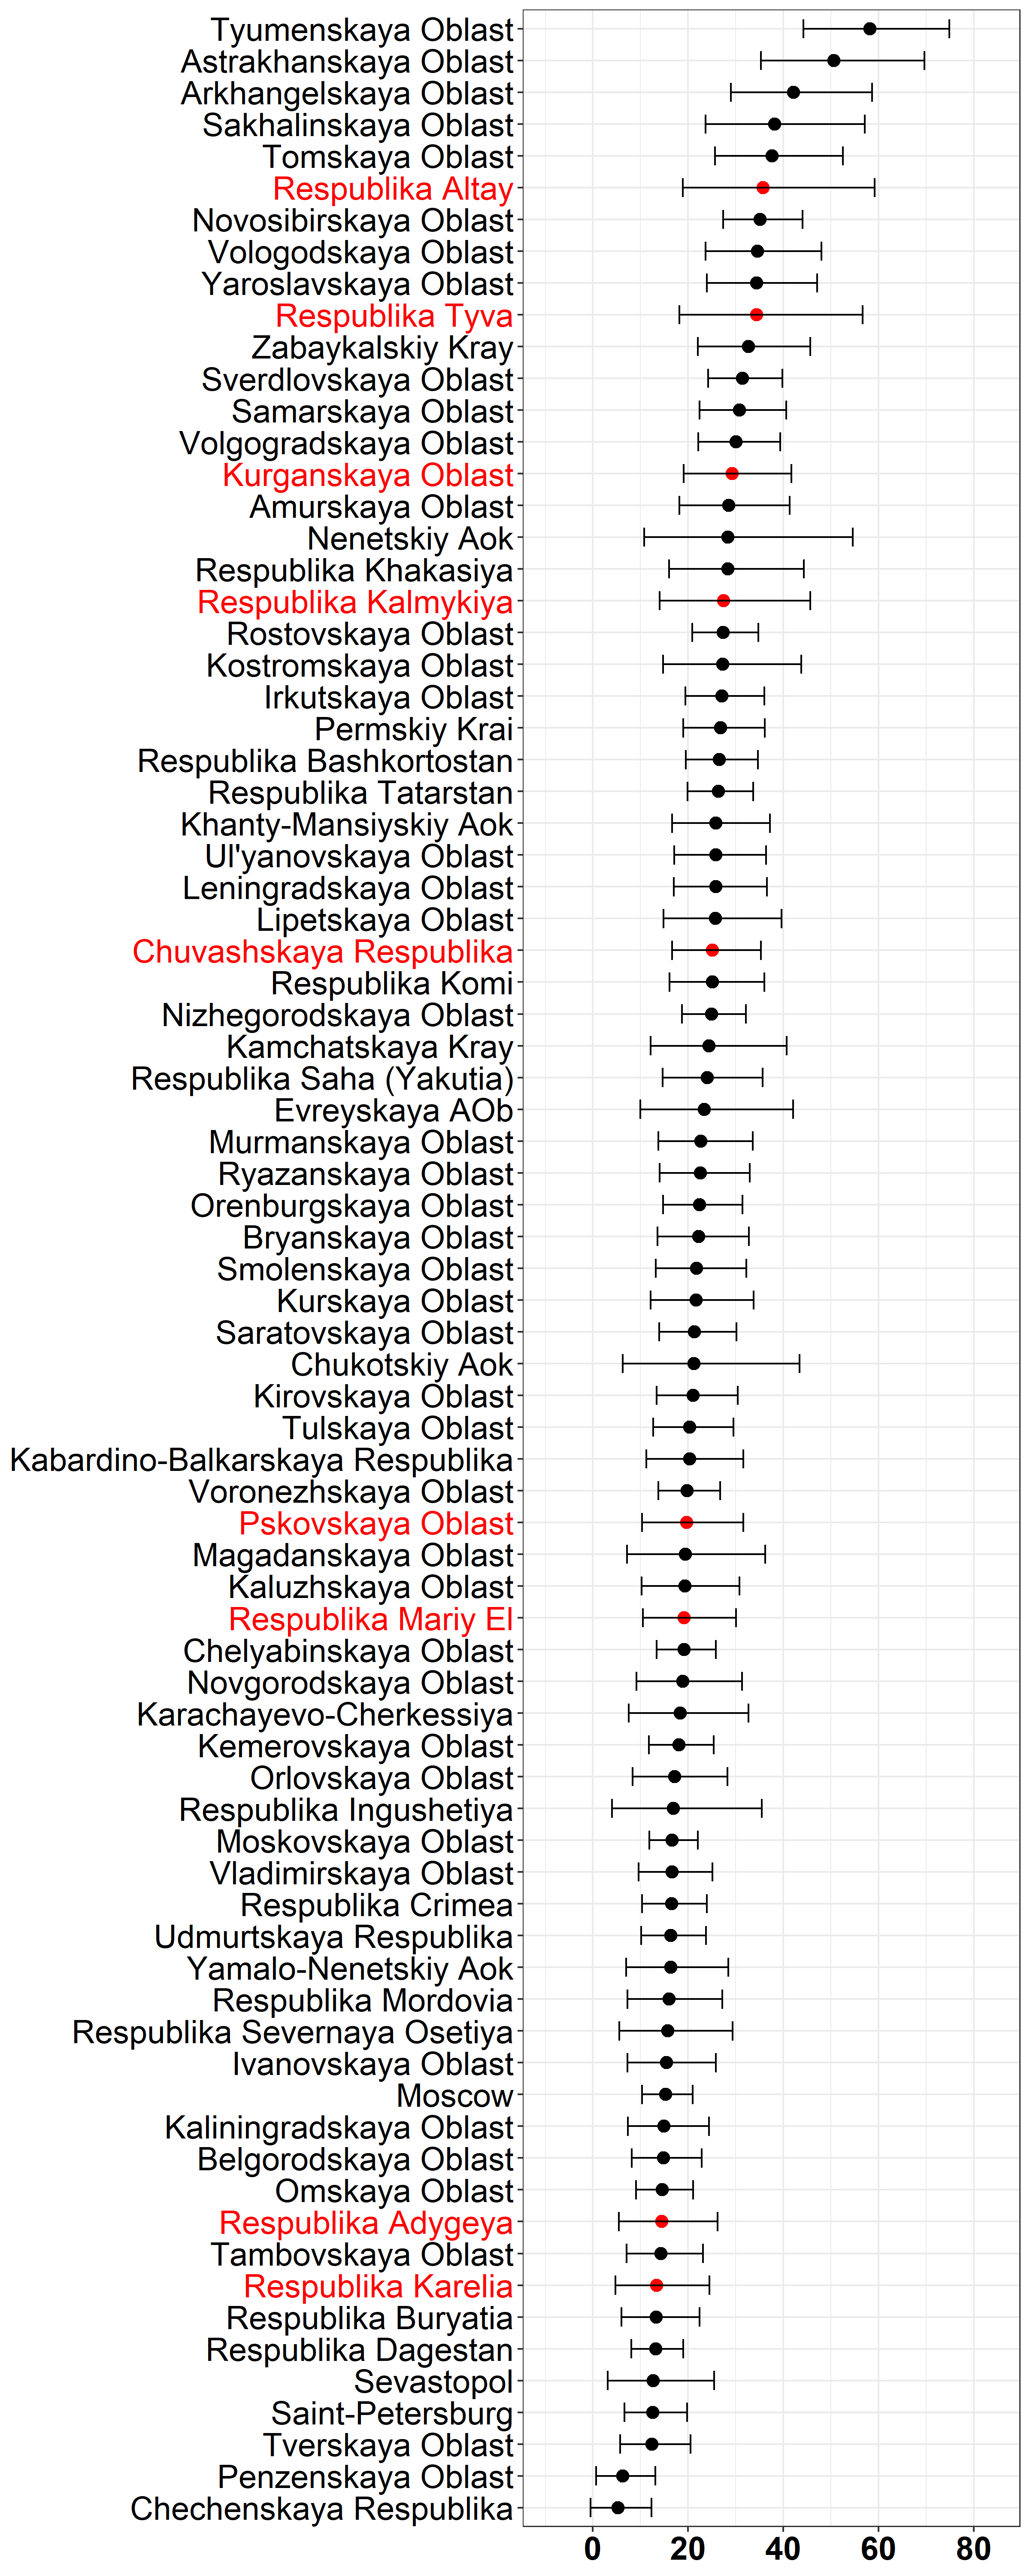
\includegraphics[width=250pt]{reg_he_18.png}
		% plot 1
		\subcaption{Higher Education \hspace{10em}   \textbf{Figure 
		1.1}}\label{}
	\end{minipage}
	\hfill
	\begin{minipage}[b]{.5\linewidth}
		\centering
		\hspace*{-0.2in}
		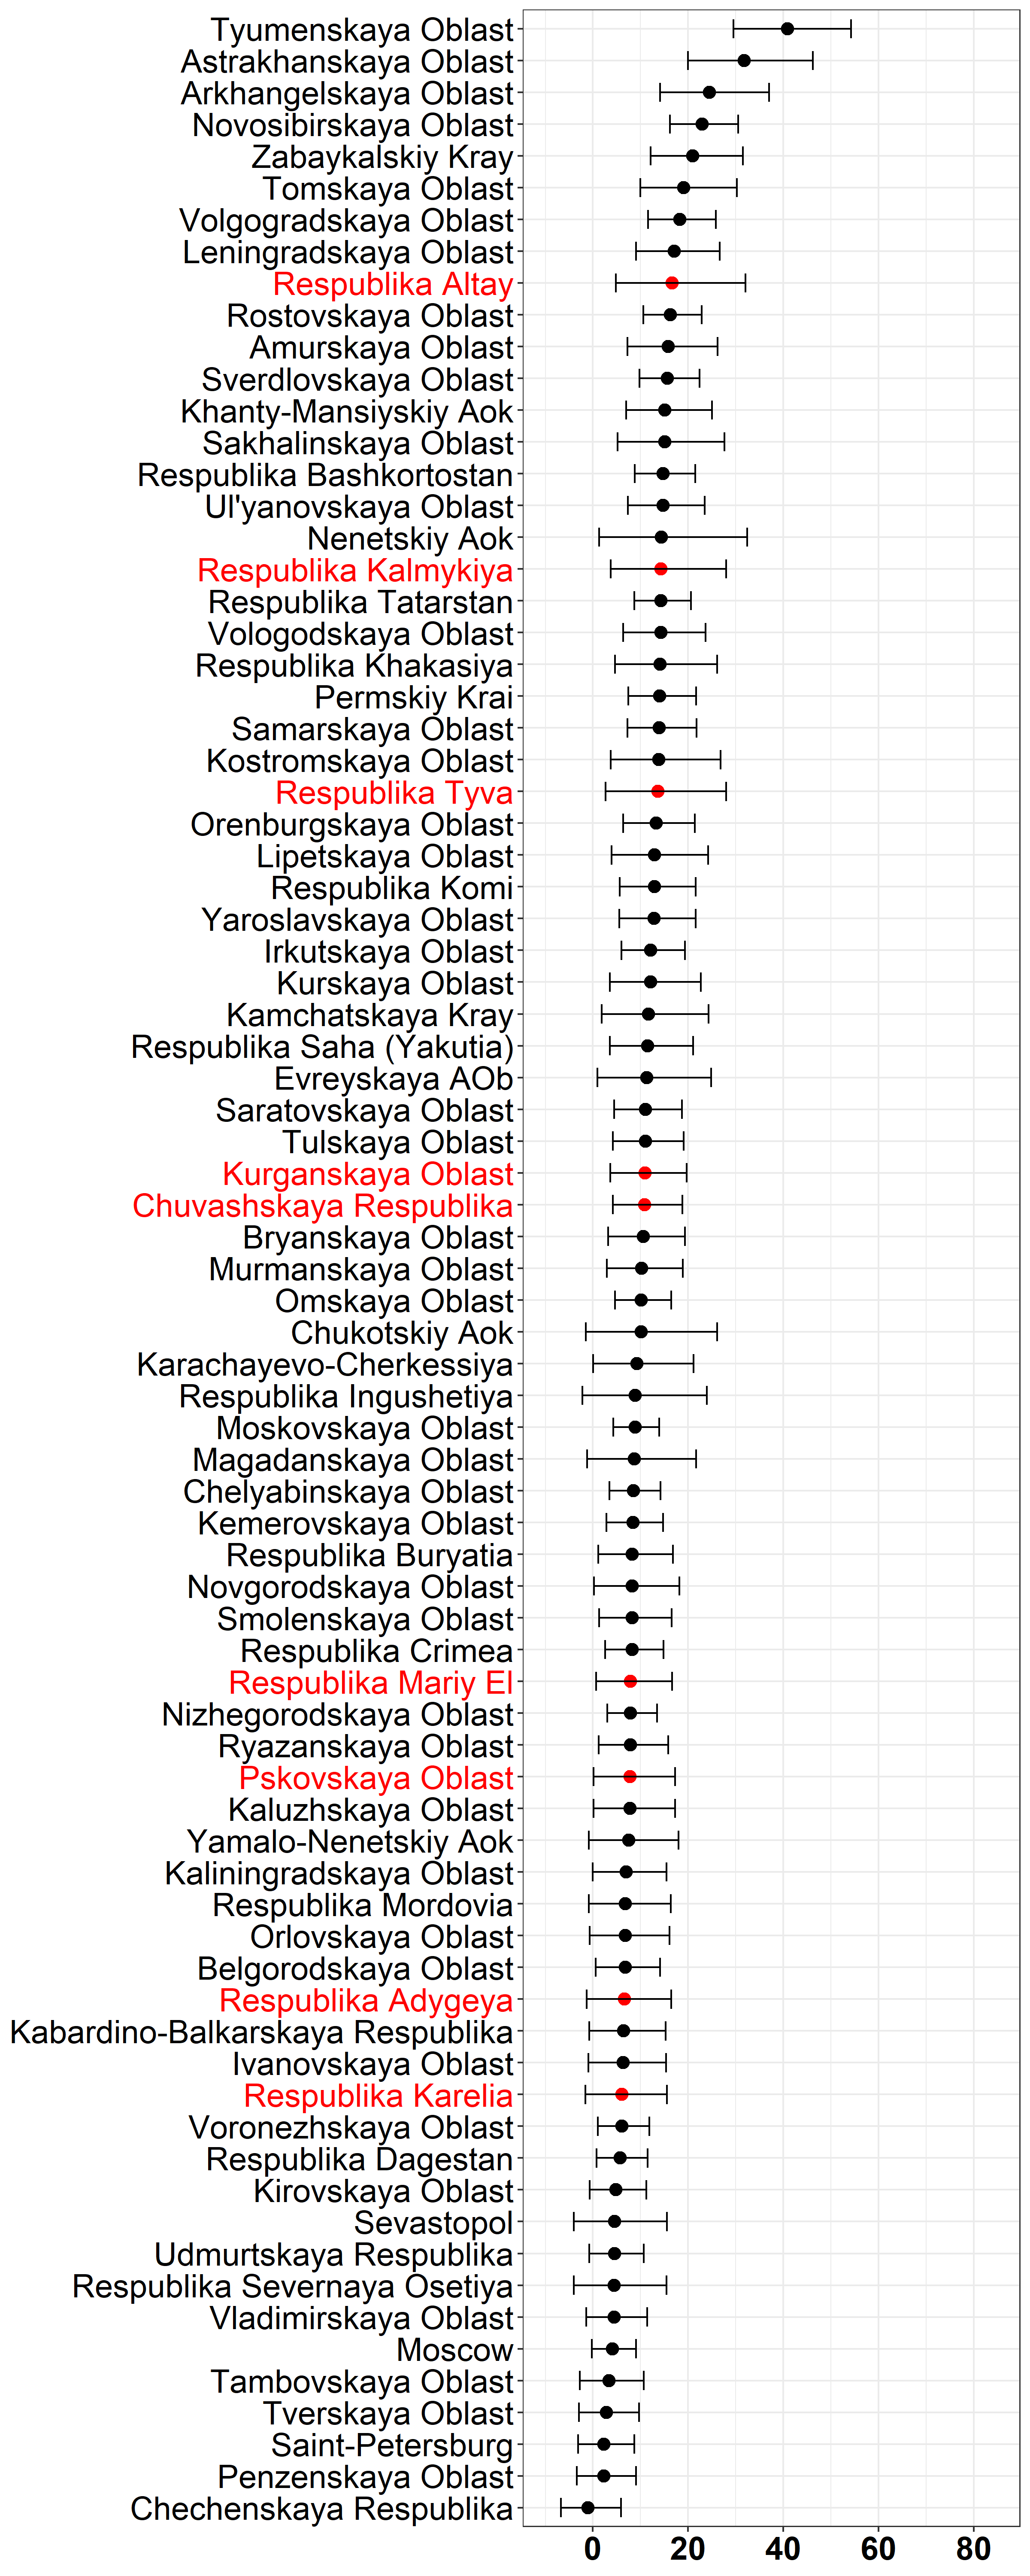
\includegraphics[width=250pt]{reg_ve_18.png}
		% plot 2
		\subcaption{Vocational Education}\label{}
	\end{minipage}
	\caption{Rates of Returns (Percentages) to Higher and Vocational Education in Russian Regions, Rosstat 2018}\label{fig:4.1}
\end{figure}


\section{Categorization of Priority Regions} 

The Presidential Executive Order on National Goals and Strategic Objectives of the Russian Federation (2018-2024) defined in December 2018 a set of 13 National Projects and 9 National Development Goals with a budget of nearly 26 trillion rubles for a six-year period. This substantive amount is the equivalent of 17\% of GDP every year. The national goals include cutting poverty by half by 2024, to improve housing conditions for 5 million people annually and to improve life expectancy. Given Russia's size and uneven geographic and economic conditions, the success of the strategic goal depends on the implementation performance at the regional and municipal levels. A sub-national focus will enhance the probability of success of the three pillars of the country's development strategy: growth, the environment and human capital. 

The Federal Government identified ten poor regions as strategic priorities in Russia. These are the lowest ranking regions according to indicators of regional income, poverty levels, unemployment rates and investment climate: Adygea, Republic (Maykop), Pskov Oblast, Altai Krai (Barnaul), Kurgan Oblast, Kalmykia, Republic, Chuvashia, Republic, Altai, Republic, Karelia, Republic, Tyva, Republic, and Mary El, Republic. The Federal Government is working on a strategy for inclusive growth and job creation in these regions. As Human Capital is expected to be an important element of the development strategy for these regions, it will be useful to examine the variation in the rates of return to education in these ten regions. Accordingly, in Figure \ref{fig:4.1}, the names of nine of the ten regions for which data was available are highlighted in red color.  It should be recalled that these returns are not simply the OLS returns, but are calculated after aggregating the fixed and random effects taking account of regional characteristics and hence are expected to be more accurate than OLS results. The 95\% confidence intervals are also presented in the figure. The priority regions are dispersed across the distribution of the rates of return to education both for vocational and higher education. Premiums to education range from 10.1 \% (Karelia Republic) to 38.2\% (Altai Republic) for university level and from 10.4\% to 20.6\% for vocational level for the same two regions. The returns for vocational and higher education are roughly moving in step, with the exception of higher returns for higher education for Kurgansk Oblast and the Tuva Republic. 

\subsection{Quantity and Quality of Skilled Labor Supply}

In order to better place policy recommendations for regions in context of their particular situation, we devised an algorithm or heuristic to classify regions according to certain variables of interest. We identified a set of variables that capture the quantity and quality of skilled labor supply and the quantity and quality of skilled labor demand. For skilled labor supply quantity, we utilized the  proportion of the labor force with a higher education degree and for skilled labor supply quality we utilized the mean university entrance exam (EGE) score for the region. Both of these are proxy variables for underlying constructs. In order to have a reasonable comparison across dimensions, the variables were standardized. In the case of the EGE score, we standardized the score to 500 for the mean for all of the Russian Federation and 100 standard deviation. For all other variables we use a mean 0 and standard deviation of 1. The plot of regions according to the two dimensions of labor supply quantity and quality is presented in Panel (a) of Figure \ref{fig:4.2}. Four regions are outliers and are not seen in the graph - St. Petersburg and Moscow in Quadrant I  and Ingushetiya Republic and Karachayevo-Cherkessiya in Quadrant IV. The graph also presents the numbers of regions in each of the quadrants. Quadrant membership, or tags from quadrants is the central piece of our classification of regions.

\subsection{Quantity and Quality of Labor Demand}

To match the classification of regions by quantity and quality of labor supply, we also carry out a similar classification for labor demand. For the quantity dimension of labor demand, we use the total share of set of specific industries in the regional GRP from Rosstat (latest available figures). We include the industries that are likely to contribute most in terms of labor force demand, excluding the oil and gas industry and excluding the mostly public sector education and health sectors. The objective is to arrive at a qualitative grouping of regions, but future research can also test sensitivity of the classification to alternative choices of sectors. The sectors chosen for this purpose were: agriculture, hunting, forestry, fishery and fish breeding, manufacturing, wholesale, retail trade and repair services, hotels and restaurants, transport and communications. The percentage contribution to GDP for these sectors by region ranged from 35\% (Tuva Republic) to 81\% (Khanty-Mansisk). 

As a measure of quality of labor demand we utilize an indicator of product 
complexity computed by \cite{lyubimov2018}. This paper is based on a 
methodology that was initially proposed and implemented by the economists 
Ricardo Hausmann and C\'{e}esar Hidalgo to capture the productive potential 
of an economy on the basis of the diversity of its products and exports 
\parencite{hausmann2011, hausmann2014}. \cite{lyubimov2018} develop an 
``Economic Complexity Index'' (ECI) utilizing production as well as export 
data. It is possible to explain intuitively the conceptualization of the 
complexity index on the basis of product diversity and the export basket. 
When we compare less developed economies with more developed ones, we see 
that more developed economies are able to manufacture a more diverse range 
of products because they have stronger production networks. Also, given the 
competitive international marketplace, the quality of products can be 
gauged by the prevalence of that product in the mix of traded goods. This 
method takes care of two problems - if a country has high exports of 
commodities, example from natural resource extraction, it does not score 
high on diversity; and if a country does manufacture a diverse range of 
goods, but these are not internationally competitive, it would also get a 
low score. \cite{lyubimov2018} extend the logic to regional measures of 
complexity. As human capital quality is closely linked to the complexity of 
products, the ECI is a very useful variable for purposes of classification 
of regions. The position of regions along the two standardized dimensions 
is shown in Panel (b) of Figure \ref{fig:4.2}.


\begin{figure}[htbp!]
	\begin{minipage}[b]{.5\linewidth}
		\centering
		#\hspace*{-0.2in}
		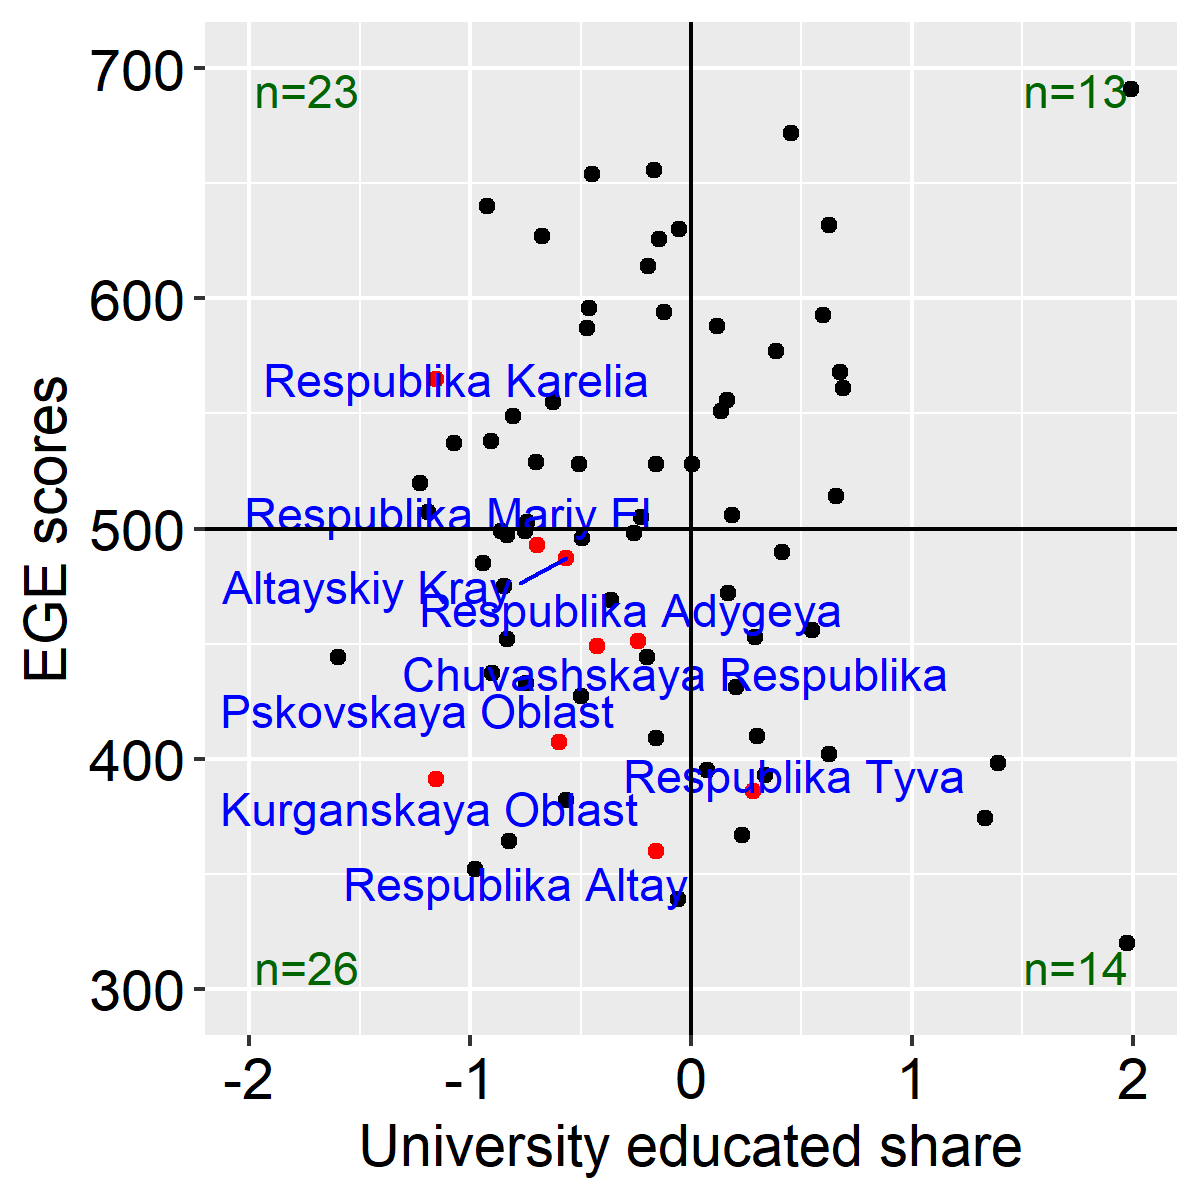
\includegraphics[width=175pt]{ranks1a.png}
		% plot 1
		\subcaption{\large{Labor Supply}}
	\end{minipage}
	\hfill
	\begin{minipage}[b]{.5\linewidth}
		\centering
		#\hspace*{-0.2in}
		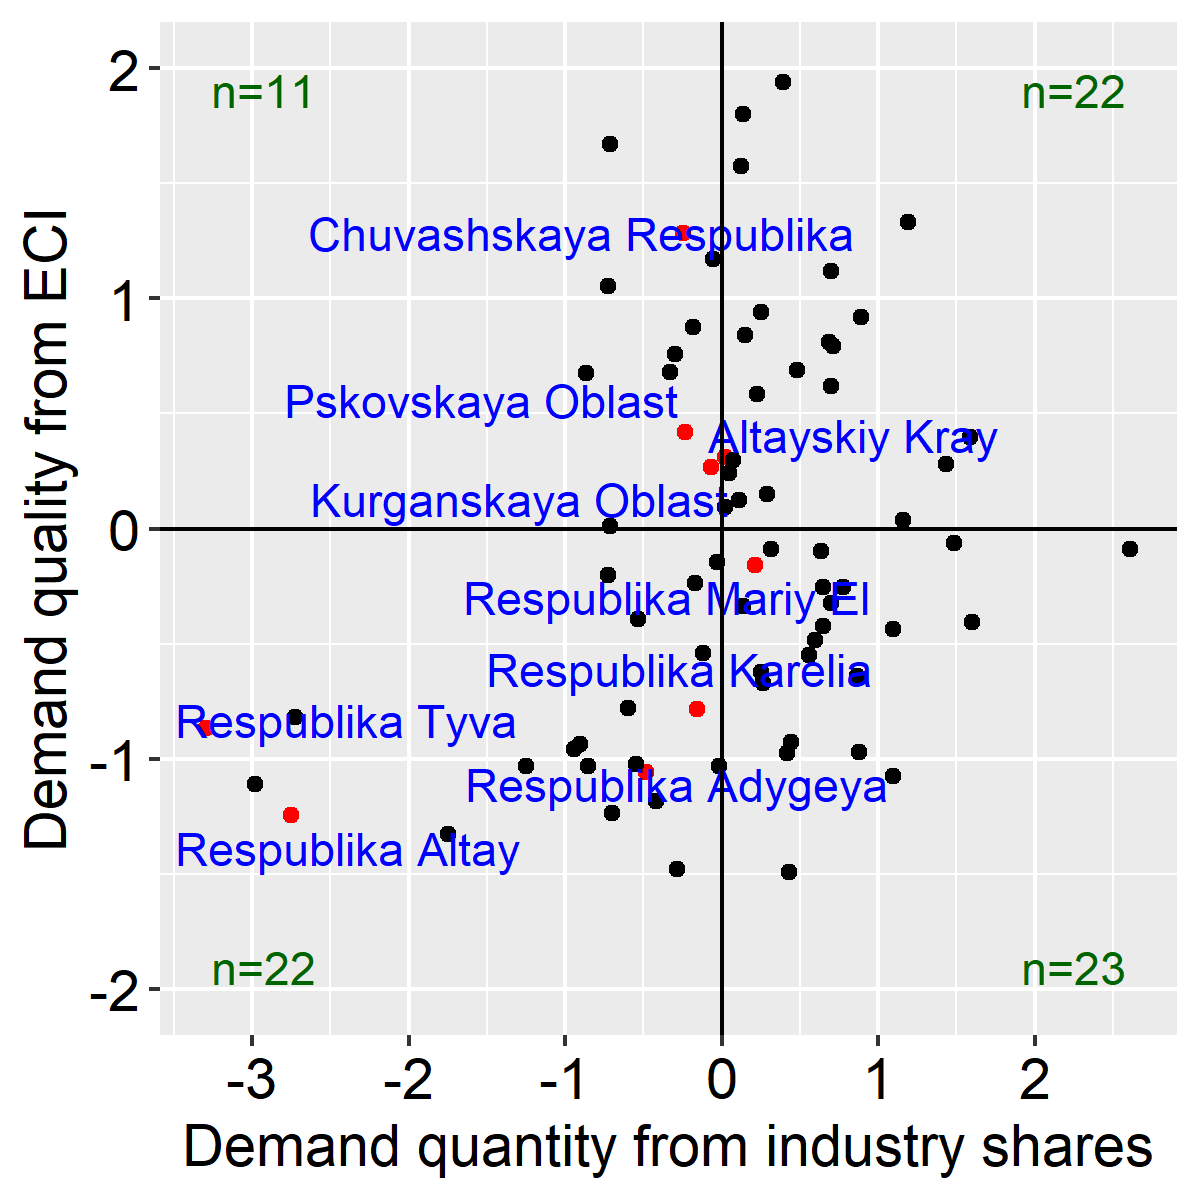
\includegraphics[width=175pt]{ranks1b.png}
		% plot 2
		\subcaption{\large{Labor Demand}}
	\end{minipage}
	\caption{Ranking of Regions on Quantity and Quality dimensions}\label{fig:4.2}
\end{figure}


\subsection{Bringing Demand and Supply classification together}

The purpose of classifying regions according to proximate measures of labor demand and labor supply is to situate the variation in regional returns to education in context. We seek to combine the quadrant classification displayed in Figure \ref{fig:4.2} with the pattern regarding returns to education. In order to do so, we compare a region's position in the demand panel on the left hand side and the supply panel on the right hand side. If a region is better placed on the demand dimension than it is with regard to the supply dimension, we term it as demand dominated; and vice versa. With four quadrants for each of the classifications, there are 4 times 4 or 16 categories that need to be simplified into 2 groups (supply or demand dominated). The decision is straightforward when a region is high on both quality and quantity of demand parameters (Quadrant I in Panel (a)) or low on both quality and quantity of supply parameters (Quadrant IV in Panel (b)). In case of ties, for 28 of the 80 regions with available data, we use the quality dimension to break ties.

We also generate a two-fold classification of the returns to education, using the classification of regions above and below the median for both returns to higher education and returns to vocational education for each region, presented in Figure \ref{fig:1.1}. When reducing from four dimensions to two, we use the returns to higher education to break ties. The result of this heuristic is a combined table that examines the returns to education in the context of labor supply or demand dominance. The classification is presented in \ref{fig:3.1} for the 80 regions for which data was available, with the priority regions highlighted using red color for the region names. Even though the priority regions are economically disadvantaged, it is very useful to note how they are spread across the four cell of Figure \ref{fig:3.1}. Policy analysis to aid development of strategies for the regions will benefit from the kind of analysis presented in this paper and even more fine-tuned analysis in the future for devising policies for specific regions. 

\vspace{-0.2in}

\begin{center}
	\begin{figure}[htbp!]
\begin{minipage}[b]{1\linewidth}
			\centering
			\hspace*{-0.3in}
			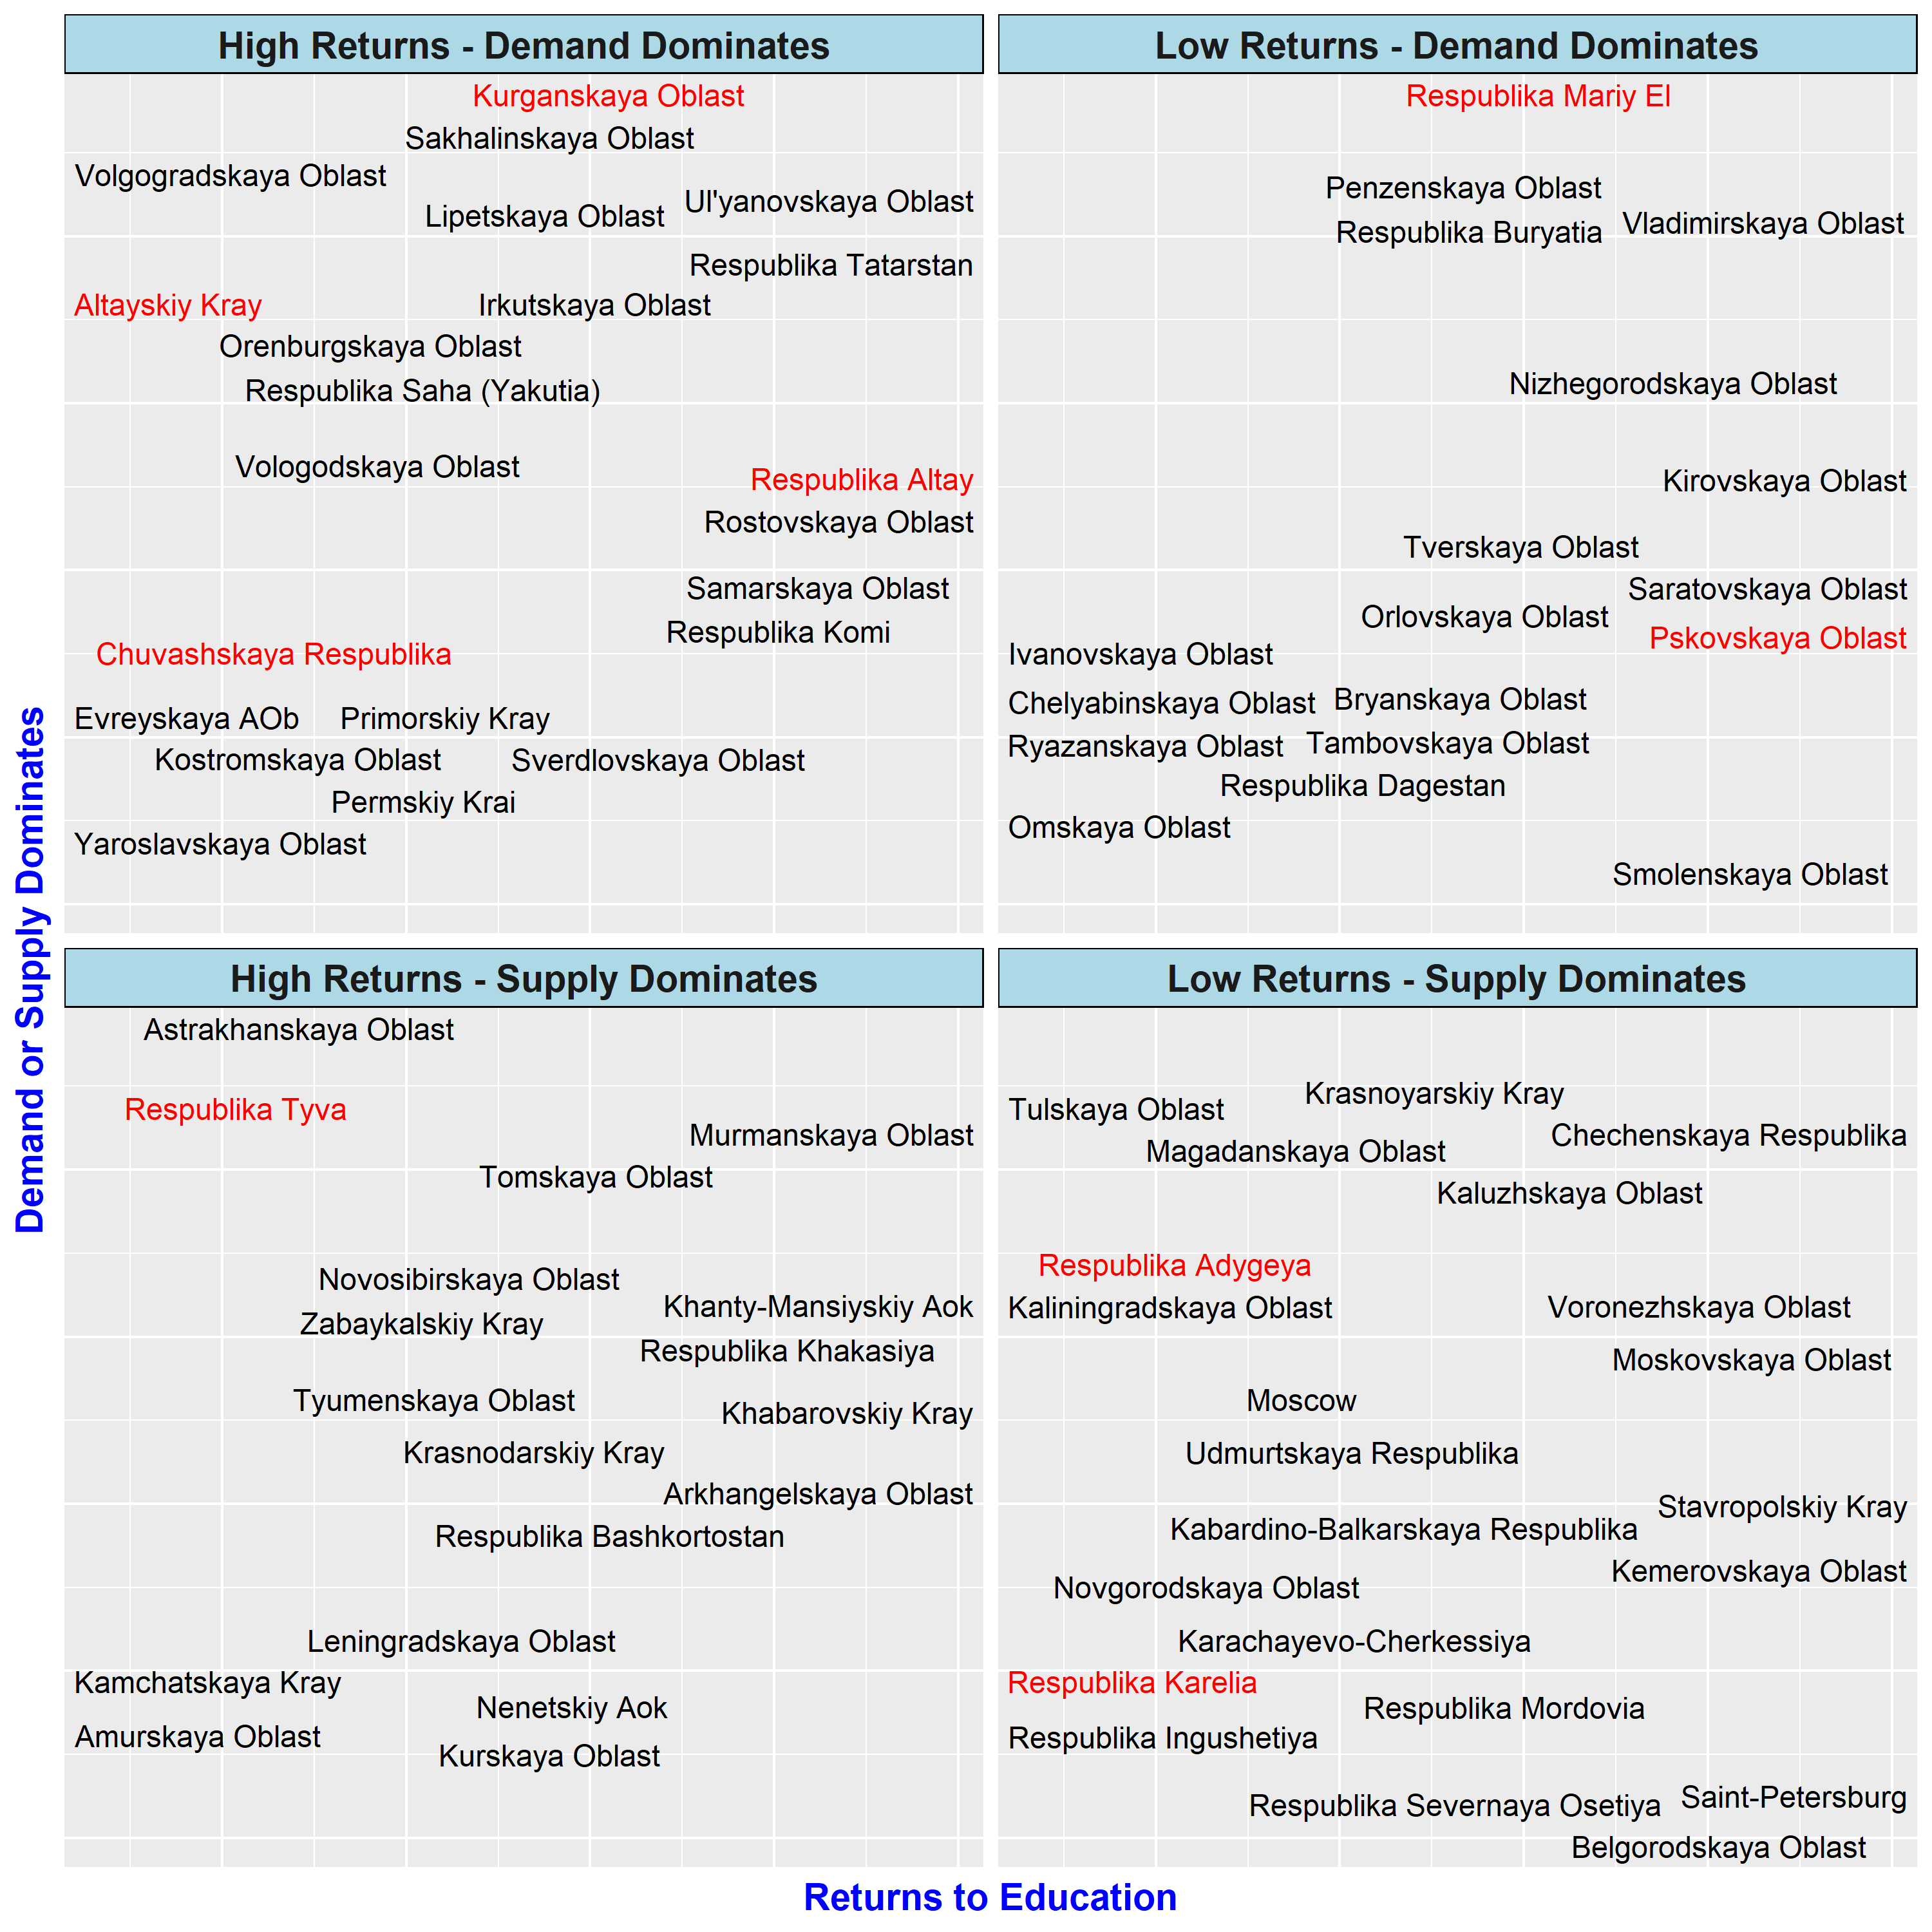
\includegraphics[width=6in]{ranks2a.png}
			% plot 1
		\end{minipage}
			\caption{Variation of Education Returns and Regional Labor Market Context}\label{fig:3.1}
	\end{figure}
\end{center}

\vspace{-2em}


\section{Policy Recommendations for Priority Regions} 

\vspace{-1em}

Returns to education tend to fall with level of economic development when comparing across countries \parencite{Psacharopoulos_Patrinos2018}. When examining the case of differential returns within the Russian Federation, we do find that St. Petersburg and Moscow city figure in the ranks of low returns. However, as studied by \cite{lyubimov2018}, the more well-off regions in the Russian Federation as well as the no so well-off regions are diverse in the make-up of their productive networks. We attempt to exploit this diversity to come up with tailored policy recommendations for regions. These are preliminary and demonstrative recommendations for groups of regions. Further analysis would need to be carried out for a specific region as the grouping used here is quite wide. For sake of brevity the analysis presented here combines the findings regarding returns to higher education and returns to vocational education, but it would be beneficial to separate them for a more granular view. 

The Table \ref{tab:4.0} provides an indicative list of policies that would be useful on the basis of an examination of the returns to education and the context of a region. Higher returns in general indicate the scope for greater investment in the supply or quantity of education as more people would be attracted to obtain higher levels of education. Lower returns to education indicate a scope for increased investment in the quality of education provision, and making better industry-education connections in terms of skills provided. When labor supply conditions are relatively good and labor demand conditions are lagging from other regions, it is an indication towards job creation policies, through innovation and entrepreneurship. When labor demand conditions are dominant, it would be an indication for better matching between jobs and skills, innovation to enhance labor productivity and diversify educational offerings. Other things constant, one would expect returns to be high when labor demand conditions are dominant and competition between employers drive up wages. However, as other things change with regional diversity, we find cases where labor supply is dominant at the same time as returns are high. With better availability of data at the regional level in the future, it would be feasible to come up with better targeted policy decision making.

\vspace{-1em}

\begin{table}[htbp!]
\centering
\renewcommand{\arraystretch}{1.5}
\setlength{\tabcolsep}{0.5em} % for the horizontal padding
	\caption{Policies fitting Regional Context}
		\label{tab:4.0}\\
\begin{tabularx}{\textwidth}{|p{20mm}|X@{}|X@{}|}
\hline
  & \textbf{High Returns to Education} & \textbf{Low Returns to Education} \\ \hline 
\textbf{Labor Demand dominates Labor Supply}
&
\begin{tabitemize}
\item Improved career guidance for high school graduates
\item Policies to encourage deeper teacher professional development in general and university education
\item Investments and policies on the industrial side � private sector firm formation; diversification or cluster specialization etc. 

\end{tabitemize}
&
\begin{tabitemize}
\item Policies to improve quality of professional colleges, higher investment in World Skills
\item Deepen supply of extra-curricular activities for better soft-skills
\item Investments in general education and policies to improve quality of provision of general education so students come out with skills needed by the market

\end{tabitemize} \\ \hline
\textbf{Labor Supply dominates Labor Demand}
&
\begin{tabitemize}
\item Policies to develop entrepreneurship and encourage job creation, including innovation policies
\item Policies to develop problem solving skills and financial literacy, including strengthening extra-curricular education
\item Investments in university quality, e.g. internationalization of universities
\end{tabitemize}
&
\begin{tabitemize}
\item Policies to integrate industries to become part of global value chains, support specific industry clusters 
\item Policies for dissemination and connectivity of educational systems like university� consortiums
\item Investments in industrial development, identification of economic activities for which region may have comparative advantage
\end{tabitemize} \\ \hline
\end{tabularx}
\end{table}


\newpage

\printbibliography

\newpage
\section*{Appendix}
\addcontentsline{toc}{section}{Appendix}%

\setcounter{table}{0}
\renewcommand{\thetable}{A\arabic{table}}

\setcounter{figure}{0}
\renewcommand{\thefigure}{A\arabic{figure}}

\hspace{-1in}
\fontsize{9}{11}{
	\selectfont
	\setlength{\tabcolsep}{2pt}
	\begin{longtable}{lcccccccccc}
		\caption{Descriptive Statistics for Regions in Russia, Rosstat 2018}
		\label{tab:4.1}\\
&  & \multicolumn{2}{c}{\textbf{Wage}} & \multicolumn{2}{c}{\textbf{Experience}} & \multicolumn{3}{c}{\textbf{Education}, \%} & \multicolumn{2}{c}{\textbf{Gender}, \%} \\ 
	    \hline
Regions & N & mean & sd & mean & sd & SE & VE & HE & Males & Females  \\
		\hline
		\endhead
		Altayskiy Kray  & $\phantom{0}4646$ & $22127.6$ & $11952.2$ & $\phantom{000}23.6$ & $\phantom{000}11.0$ & $17.456$ & $54.50$ & $28.05$ & $48.90$ & $51.10$ \\
		Amurskaya Oblast  & $\phantom{0}2557$ & $33441.2$ & $17409.0$ & $\phantom{000}23.2$ & $\phantom{000}11.2$ & $16.347$ & $50.65$ & $33.01$ & $49.59$ & $50.41$ \\
		Arkhangelskaya Oblast  & $\phantom{0}3183$ & $33438.1$ & $16884.2$ & $\phantom{000}22.6$ & $\phantom{000}10.6$ & $12.692$ & $54.95$ & $32.36$ & $44.17$ & $55.83$ \\
		Astrakhanskaya Oblast  & $\phantom{0}2836$ & $26474.1$ & $13737.6$ & $\phantom{000}23.0$ & $\phantom{000}11.3$ & $13.646$ & $55.08$ & $31.28$ & $50.99$ & $49.01$ \\
		Belgorodskaya Oblast  & $\phantom{0}3692$ & $26281.0$ & $10811.9$ & $\phantom{000}23.8$ & $\phantom{000}11.1$ & $12.351$ & $54.47$ & $33.18$ & $49.76$ & $50.24$ \\
		Bryanskaya Oblast  & $\phantom{0}3087$ & $22482.3$ & $\phantom{0}9634.1$ & $\phantom{000}23.5$ & $\phantom{000}10.9$ & $19.631$ & $50.66$ & $29.71$ & $48.66$ & $51.34$ \\
		Chechenskaya Respublika  & $\phantom{0}2010$ & $27718.4$ & $11793.2$ & $\phantom{000}18.7$ & $\phantom{000}10.6$ & $25.721$ & $26.37$ & $47.91$ & $65.37$ & $34.63$ \\
		Chelyabinskaya Oblast  & $\phantom{0}6717$ & $27990.8$ & $14280.9$ & $\phantom{000}23.9$ & $\phantom{000}11.2$ & $12.104$ & $54.53$ & $33.36$ & $47.39$ & $52.61$ \\
		Chukotskiy Aok  & $\phantom{0}1535$ & $65574.1$ & $32370.8$ & $\phantom{000}23.6$ & $\phantom{000}10.6$ & $13.941$ & $46.06$ & $40.00$ & $43.97$ & $56.03$ \\
		Chuvashskaya Respublika  & $\phantom{0}3248$ & $21453.7$ & $12602.2$ & $\phantom{000}24.3$ & $\phantom{000}11.0$ & $19.119$ & $50.80$ & $30.08$ & $50.18$ & $49.82$ \\
		Evreyskaya AOb  & $\phantom{0}1536$ & $28532.1$ & $17385.1$ & $\phantom{000}23.8$ & $\phantom{000}11.2$ & $22.005$ & $50.33$ & $27.67$ & $50.00$ & $50.00$ \\
		Irkutskaya Oblast  & $\phantom{0}4686$ & $29967.6$ & $17443.1$ & $\phantom{000}22.3$ & $\phantom{000}11.2$ & $17.520$ & $47.06$ & $35.42$ & $47.57$ & $52.43$ \\
		Ivanovskaya Oblast  & $\phantom{0}2876$ & $24881.8$ & $12496.8$ & $\phantom{000}23.3$ & $\phantom{000}10.9$ & $20.341$ & $49.90$ & $29.76$ & $47.77$ & $52.23$ \\
		Kabardino-Balkarskaya Res.  & $\phantom{0}2006$ & $23592.3$ & $10766.2$ & $\phantom{000}21.7$ & $\phantom{000}11.6$ & $21.137$ & $40.53$ & $38.33$ & $52.04$ & $47.96$ \\
		Kaliningradskaya Oblast  & $\phantom{0}2838$ & $29749.2$ & $15489.1$ & $\phantom{000}23.5$ & $\phantom{000}11.4$ & $13.495$ & $52.40$ & $34.11$ & $50.07$ & $49.93$ \\
		Kaluzhskaya Oblast  & $\phantom{0}3155$ & $29662.1$ & $12879.5$ & $\phantom{000}24.1$ & $\phantom{000}11.2$ & $13.312$ & $52.11$ & $34.58$ & $47.92$ & $52.08$ \\
		Kamchatskaya Kray  & $\phantom{0}2203$ & $51160.5$ & $29997.7$ & $\phantom{000}23.1$ & $\phantom{000}11.2$ & $13.118$ & $42.99$ & $43.89$ & $47.89$ & $52.11$ \\
		Karachayevo-Cherkessiya  & $\phantom{0}1510$ & $22900.6$ & $12540.8$ & $\phantom{000}22.0$ & $\phantom{000}11.8$ & $17.152$ & $40.07$ & $42.78$ & $48.01$ & $51.99$ \\
		Kemerovskaya Oblast  & $\phantom{0}5056$ & $26287.0$ & $13774.4$ & $\phantom{000}23.6$ & $\phantom{000}11.3$ & $18.137$ & $52.99$ & $28.88$ & $48.04$ & $51.96$ \\
		Khabarovskiy Kray  & $\phantom{0}3731$ & $42008.8$ & $21837.8$ & $\phantom{000}22.3$ & $\phantom{000}11.2$ & $11.900$ & $44.33$ & $43.77$ & $46.15$ & $53.85$ \\
		Khanty-Mansiyskiy Aok  & $\phantom{0}4335$ & $50837.9$ & $22261.7$ & $\phantom{000}22.8$ & $\phantom{000}10.5$ & $13.564$ & $46.78$ & $39.65$ & $49.60$ & $50.40$ \\
		Kirovskaya Oblast  & $\phantom{0}3284$ & $22941.0$ & $13674.6$ & $\phantom{000}25.1$ & $\phantom{000}11.2$ & $20.128$ & $55.33$ & $24.54$ & $47.69$ & $52.31$ \\
		Kostromskaya Oblast  & $\phantom{0}2518$ & $23993.1$ & $12090.9$ & $\phantom{000}23.6$ & $\phantom{000}11.1$ & $12.669$ & $61.28$ & $26.05$ & $47.82$ & $52.18$ \\
		Krasnodarskiy Kray  & $\phantom{0}8730$ & $32563.7$ & $17499.8$ & $\phantom{000}23.0$ & $\phantom{000}10.9$ & $15.888$ & $48.57$ & $35.54$ & $50.02$ & $49.98$ \\
		Krasnoyarskiy Kray  & $\phantom{0}5540$ & $33954.6$ & $21199.2$ & $\phantom{000}23.0$ & $\phantom{000}11.0$ & $21.588$ & $48.05$ & $30.36$ & $49.64$ & $50.36$ \\
		Kurganskaya Oblast  & $\phantom{0}2468$ & $20896.9$ & $11539.5$ & $\phantom{000}24.4$ & $\phantom{000}10.7$ & $21.394$ & $52.47$ & $26.13$ & $48.38$ & $51.62$ \\
		Kurskaya Oblast  & $\phantom{0}2956$ & $23622.6$ & $11475.0$ & $\phantom{000}23.9$ & $\phantom{000}11.0$ & $14.783$ & $52.17$ & $33.05$ & $50.30$ & $49.70$ \\
		Leningradskaya Oblast  & $\phantom{0}4506$ & $32124.3$ & $17227.4$ & $\phantom{000}24.2$ & $\phantom{000}11.5$ & $\phantom{0}7.723$ & $54.77$ & $37.51$ & $46.03$ & $53.97$ \\
		Lipetskaya Oblast  & $\phantom{0}2869$ & $25037.8$ & $10813.5$ & $\phantom{000}24.1$ & $\phantom{000}11.0$ & $13.106$ & $53.82$ & $33.08$ & $49.60$ & $50.40$ \\
		Magadanskaya Oblast  & $\phantom{0}1841$ & $51000.8$ & $23729.4$ & $\phantom{000}24.1$ & $\phantom{000}11.4$ & $18.523$ & $43.02$ & $38.46$ & $43.24$ & $56.76$ \\
		Moscow  & $29921$ & $66263.5$ & $26437.9$ & $\phantom{000}20.8$ & $\phantom{000}10.8$ & $\phantom{0}4.953$ & $32.18$ & $62.86$ & $47.06$ & $52.94$ \\
		Moskovskaya Oblast  & $13431$ & $46725.1$ & $20563.7$ & $\phantom{000}22.6$ & $\phantom{000}11.4$ & $10.975$ & $39.13$ & $49.89$ & $47.51$ & $52.49$ \\
		Murmanskaya Oblast  & $\phantom{0}3078$ & $43992.5$ & $28841.9$ & $\phantom{000}23.4$ & $\phantom{000}11.2$ & $12.801$ & $50.45$ & $36.74$ & $49.84$ & $50.16$ \\
		Nenetskiy Aok  & $\phantom{0}1118$ & $54467.3$ & $23147.1$ & $\phantom{000}22.6$ & $\phantom{000}10.8$ & $17.263$ & $49.73$ & $33.01$ & $39.98$ & $60.02$ \\
		Nizhegorodskaya Oblast  & $\phantom{0}6139$ & $30912.9$ & $13291.8$ & $\phantom{000}23.4$ & $\phantom{000}11.2$ & $16.941$ & $49.31$ & $33.75$ & $47.42$ & $52.58$ \\
		Novgorodskaya Oblast  & $\phantom{0}2673$ & $26856.0$ & $12683.0$ & $\phantom{000}24.6$ & $\phantom{000}11.2$ & $15.638$ & $55.74$ & $28.62$ & $45.16$ & $54.84$ \\
		Novosibirskaya Oblast  & $\phantom{0}5374$ & $29229.9$ & $14687.7$ & $\phantom{000}23.9$ & $\phantom{000}11.6$ & $16.561$ & $49.33$ & $34.11$ & $47.06$ & $52.94$ \\
		Omskaya Oblast  & $\phantom{0}3978$ & $25337.5$ & $14613.1$ & $\phantom{000}23.6$ & $\phantom{000}10.9$ & $22.197$ & $51.31$ & $26.50$ & $51.11$ & $48.89$ \\
		Orenburgskaya Oblast  & $\phantom{0}4190$ & $24207.0$ & $12519.9$ & $\phantom{000}23.3$ & $\phantom{000}11.0$ & $15.131$ & $53.68$ & $31.19$ & $51.29$ & $48.71$ \\
		Orlovskaya Oblast  & $\phantom{0}2424$ & $21901.2$ & $10561.0$ & $\phantom{000}24.7$ & $\phantom{000}11.1$ & $15.017$ & $50.66$ & $34.32$ & $46.99$ & $53.01$ \\
		Penzenskaya Oblast  & $\phantom{0}3103$ & $23478.4$ & $10982.9$ & $\phantom{000}24.2$ & $\phantom{000}11.0$ & $20.722$ & $51.40$ & $27.88$ & $51.02$ & $48.98$ \\
		Permskiy Krai  & $\phantom{0}5290$ & $29176.6$ & $14449.4$ & $\phantom{000}23.4$ & $\phantom{000}11.0$ & $13.894$ & $58.32$ & $27.79$ & $48.17$ & $51.83$ \\
		Primorskiy Kray  & $\phantom{0}4104$ & $37839.9$ & $18420.2$ & $\phantom{000}23.8$ & $\phantom{000}11.3$ & $14.985$ & $52.97$ & $32.04$ & $49.98$ & $50.02$ \\
		Pskovskaya Oblast  & $\phantom{0}2382$ & $23838.4$ & $12015.3$ & $\phantom{000}25.0$ & $\phantom{000}11.0$ & $17.632$ & $55.33$ & $27.04$ & $48.11$ & $51.89$ \\
		Respublika Adygeya  & $\phantom{0}2013$ & $21350.3$ & $10505.9$ & $\phantom{000}23.4$ & $\phantom{000}11.3$ & $20.666$ & $43.67$ & $35.67$ & $49.53$ & $50.47$ \\
		Respublika Altay  & $\phantom{0}1381$ & $20285.3$ & $12029.5$ & $\phantom{000}23.0$ & $\phantom{000}10.6$ & $23.027$ & $45.26$ & $31.72$ & $43.08$ & $56.92$ \\
		Respublika Bashkortostan  & $\phantom{0}7126$ & $31100.8$ & $15175.2$ & $\phantom{000}23.4$ & $\phantom{000}11.0$ & $12.167$ & $56.67$ & $31.17$ & $51.98$ & $48.02$ \\
		Respublika Buryatia  & $\phantom{0}2469$ & $29536.3$ & $17237.4$ & $\phantom{000}22.1$ & $\phantom{000}10.6$ & $17.173$ & $45.61$ & $37.22$ & $48.12$ & $51.88$ \\
		Respublika Dagestan  & $\phantom{0}3388$ & $26377.3$ & $11971.9$ & 
		$\phantom{000}23.0$ & $\phantom{000}10.7$ & $30.519$ & $30.79$ & 
		$38.70$ & $55.99$ & $44.01$ \\
		Respublika Ingushetiya  & $\phantom{0}1207$ & $23740.2$ & $10168.5$ & $\phantom{000}18.2$ & $\phantom{0000}9.6$ & $10.025$ & $18.89$ & $71.09$ & $61.14$ & $38.86$ \\
		Respublika Kalmykiya  & $\phantom{0}1751$ & $18568.8$ & $11749.1$ & $\phantom{000}23.6$ & $\phantom{000}11.4$ & $15.762$ & $40.89$ & $43.35$ & $46.43$ & $53.57$ \\
		Respublika Karelia  & $\phantom{0}2164$ & $28510.2$ & $16639.5$ & $\phantom{000}23.7$ & $\phantom{000}10.8$ & $17.144$ & $55.45$ & $27.40$ & $47.00$ & $53.00$ \\
		Respublika Khakasiya  & $\phantom{0}2064$ & $27288.1$ & $16613.3$ & $\phantom{000}23.3$ & $\phantom{000}11.1$ & $22.045$ & $51.11$ & $26.84$ & $50.97$ & $49.03$ \\
		Respublika Komi  & $\phantom{0}2972$ & $35891.6$ & $21554.4$ & $\phantom{000}23.8$ & $\phantom{000}11.0$ & $16.689$ & $53.47$ & $29.85$ & $46.67$ & $53.33$ \\
		Respublika Mariy El  & $\phantom{0}2486$ & $21133.1$ & $11941.6$ & $\phantom{000}24.1$ & $\phantom{000}11.2$ & $18.785$ & $52.98$ & $28.24$ & $47.87$ & $52.13$ \\
		Respublika Mordovia  & $\phantom{0}2236$ & $21221.0$ & $10837.3$ & $\phantom{000}23.1$ & $\phantom{000}11.2$ & $15.519$ & $49.11$ & $35.38$ & $48.35$ & $51.65$ \\
		Respublika Saha (Yakutia)  & $\phantom{0}3243$ & $45763.1$ & $25001.6$ & $\phantom{000}23.2$ & $\phantom{000}11.3$ & $18.440$ & $45.76$ & $35.80$ & $46.69$ & $53.31$ \\
		Respublika Severnaya Osetiya  & $\phantom{0}2114$ & $22993.1$ & $12762.5$ & $\phantom{000}21.8$ & $\phantom{000}11.3$ & $12.677$ & $40.92$ & $46.40$ & $48.91$ & $51.09$ \\
		Respublika Tatarstan  & $\phantom{0}7212$ & $30327.9$ & $12928.8$ & $\phantom{000}23.5$ & $\phantom{000}11.1$ & $18.691$ & $48.64$ & $32.67$ & $51.48$ & $48.52$ \\
		Respublika Tyva  & $\phantom{0}1704$ & $23421.9$ & $16851.3$ & $\phantom{000}21.4$ & $\phantom{000}10.0$ & $19.777$ & $44.78$ & $35.45$ & $40.43$ & $59.57$ \\
		Rostovskaya Oblast  & $\phantom{0}6985$ & $28287.2$ & $12779.9$ & $\phantom{000}23.1$ & $\phantom{000}11.0$ & $15.476$ & $48.03$ & $36.49$ & $50.68$ & $49.32$ \\
		Ryazanskaya Oblast  & $\phantom{0}2609$ & $25889.2$ & $11760.9$ & $\phantom{000}24.7$ & $\phantom{000}11.1$ & $12.457$ & $59.37$ & $28.17$ & $49.18$ & $50.82$ \\
		Saint-Petersburg  & $11352$ & $48520.8$ & $23771.0$ & $\phantom{000}22.8$ & $\phantom{000}11.4$ & $\phantom{0}5.259$ & $38.15$ & $56.59$ & $46.04$ & $53.96$ \\
		Sakhalinskaya Oblast  & $\phantom{0}2258$ & $50325.1$ & $25563.0$ & $\phantom{000}23.6$ & $\phantom{000}11.2$ & $17.493$ & $48.23$ & $34.28$ & $46.94$ & $53.06$ \\
		Samarskaya Oblast  & $\phantom{0}6275$ & $32584.4$ & $15015.6$ & $\phantom{000}23.8$ & $\phantom{000}11.1$ & $11.331$ & $47.87$ & $40.80$ & $47.71$ & $52.29$ \\
		Saratovskaya Oblast  & $\phantom{0}4572$ & $23698.6$ & $12322.4$ & $\phantom{000}23.7$ & $\phantom{000}10.8$ & $14.961$ & $50.22$ & $34.82$ & $50.42$ & $49.58$ \\
		Smolenskaya Oblast  & $\phantom{0}2726$ & $25517.8$ & $12104.9$ & 
		$\phantom{000}24.6$ & $\phantom{000}11.3$ & $14.380$ & $52.31$ & 
		$33.31$ & $46.04$ & $53.96$ \\
		Stavropolskiy Kray  & $\phantom{0}4945$ & $25263.6$ & $12696.7$ & $\phantom{000}22.6$ & $\phantom{000}11.3$ & $16.946$ & $43.80$ & $39.25$ & $47.48$ & $52.52$ \\
		Sverdlovskaya Oblast  & $\phantom{0}7712$ & $35983.2$ & $15242.7$ & $\phantom{000}23.6$ & $\phantom{000}11.3$ & $16.779$ & $54.94$ & $28.28$ & $48.59$ & $51.41$ \\
		Tambovskaya Oblast  & $\phantom{0}2781$ & $22698.6$ & $10440.1$ & $\phantom{000}24.1$ & $\phantom{000}11.0$ & $16.397$ & $53.54$ & $30.06$ & $50.67$ & $49.33$ \\
		Tomskaya Oblast  & $\phantom{0}3074$ & $29580.6$ & $16745.7$ & $\phantom{000}22.1$ & $\phantom{000}11.1$ & $13.500$ & $47.56$ & $38.94$ & $46.78$ & $53.22$ \\
		Tulskaya Oblast  & $\phantom{0}3516$ & $27687.4$ & $11814.7$ & $\phantom{000}24.3$ & $\phantom{000}11.3$ & $17.491$ & $54.69$ & $27.82$ & $48.98$ & $51.02$ \\
		Tverskaya Oblast  & $\phantom{0}3157$ & $26310.0$ & $15025.1$ & $\phantom{000}25.5$ & $\phantom{000}11.1$ & $14.824$ & $56.57$ & $28.60$ & $44.73$ & $55.27$ \\
		Tyumenskaya Oblast  & $\phantom{0}3095$ & $31441.2$ & $17278.6$ & $\phantom{000}22.7$ & $\phantom{000}11.2$ & $16.123$ & $52.89$ & $30.99$ & $50.05$ & $49.95$ \\
		Udmurtskaya Respublika  & $\phantom{0}4073$ & $24044.6$ & $11540.9$ & $\phantom{000}23.9$ & $\phantom{000}11.3$ & $20.108$ & $51.04$ & $28.85$ & $46.99$ & $53.01$ \\
		Ul'yanovskaya Oblast  & $\phantom{0}3109$ & $23215.3$ & $10596.4$ & $\phantom{000}24.8$ & $\phantom{000}10.9$ & $19.170$ & $53.84$ & $26.99$ & $50.37$ & $49.63$ \\
		Vladimirskaya Oblast  & $\phantom{0}3502$ & $25001.4$ & $12605.8$ & $\phantom{000}24.5$ & $\phantom{000}11.4$ & $19.503$ & $50.77$ & $29.73$ & $46.49$ & $53.51$ \\
		Volgogradskaya Oblast  & $\phantom{0}4836$ & $24459.0$ & $12915.8$ & $\phantom{000}23.2$ & $\phantom{000}11.0$ & $15.881$ & $50.91$ & $33.21$ & $49.69$ & $50.31$ \\
		Vologodskaya Oblast  & $\phantom{0}2965$ & $28248.9$ & $16693.8$ & $\phantom{000}23.9$ & $\phantom{000}11.2$ & $17.302$ & $57.47$ & $25.23$ & $49.61$ & $50.39$ \\
		Voronezhskaya Oblast  & $\phantom{0}4348$ & $26261.9$ & $11813.9$ & $\phantom{000}23.6$ & $\phantom{000}11.5$ & $22.700$ & $43.38$ & $33.92$ & $48.37$ & $51.63$ \\
		Yamalo-Nenetskiy Aok  & $\phantom{0}3164$ & $69356.7$ & $28075.6$ & $\phantom{000}21.0$ & $\phantom{000}10.4$ & $10.683$ & $40.27$ & $49.05$ & $48.74$ & $51.26$ \\
		Yaroslavskaya Oblast  & $\phantom{0}3361$ & $30261.4$ & $14682.8$ & $\phantom{000}24.1$ & $\phantom{000}11.4$ & $16.215$ & $53.73$ & $30.05$ & $47.01$ & $52.99$ \\
		Zabaykalskiy Kray  & $\phantom{0}3017$ & $28336.6$ & $16350.4$ & $\phantom{000}23.0$ & $\phantom{000}10.6$ & $24.561$ & $47.40$ & $28.04$ & $47.07$ & $52.93$ \\
		\hline 
	\end{longtable}
}


\begin{table}[!htbp] \centering 
	\caption{} 
		\label{tab:4.2}\\
	\label{} 
	\begin{tabular}{@{\extracolsep{5pt}}lcccc} 
		\\[-1.8ex]\hline 
		\hline \\[-1.8ex] 
		& Null model & Mincerian & Random Slope & Cross-Level Interaction \\ 
		\\[-1.8ex] & (1) & (2) & (3) & (4)\\ 
		\hline \\[-1.8ex] 
		Constant & 10.178$^{***}$ & 10.032$^{***}$ & 10.056$^{***}$ & 10.065$^{***}$ \\ 
		& (0.034) & (0.034) & (0.036) & (0.036) \\ 
		& & & & \\ 
		Vocational &  & 0.283$^{***}$ & 0.279$^{***}$ & 0.267$^{***}$ \\ 
		&  & (0.009) & (0.021) & (0.021) \\ 
		& & & & \\ 
		Higher &  & 0.638$^{***}$ & 0.641$^{***}$ & 0.622$^{***}$ \\ 
		&  & (0.009) & (0.025) & (0.025) \\ 
		& & & & \\ 
		Coverage VE X Vocational &  &  &  & 0.050$^{**}$ \\ 
		&  &  &  & (0.025) \\ 
		& & & & \\ 
		Coverage VE X Higher &  &  &  & 0.083$^{***}$ \\ 
		&  &  &  & (0.030) \\ 
		& & & & \\ 
		Experience &  & $-$0.026$^{***}$ & $-$0.027$^{***}$ & $-$0.027$^{***}$ \\ 
		&  & (0.002) & (0.002) & (0.002) \\ 
		& & & & \\ 
		Experience squared &  & $-$0.065$^{***}$ & $-$0.065$^{***}$ & $-$0.065$^{***}$ \\ 
		&  & (0.002) & (0.002) & (0.002) \\ 
		& & & & \\ 
		Females &  & $-$0.403$^{***}$ & $-$0.404$^{***}$ & $-$0.404$^{***}$ \\ 
		&  & (0.005) & (0.005) & (0.005) \\ 
		& & & & \\ 
		Coverage VE &  &  & $-$0.101$^{***}$ & $-$0.142$^{***}$ \\ 
		&  &  & (0.039) & (0.043) \\ 
		& & & & \\ 
		\hline \\[-1.8ex] 
		Variance of Intecept & 0.09 & 0.08 & 0.09 & 0.09 \\ 
		Variance of Vocational &  &  & 0.02 & 0.02 \\ 
		Variance of Higher &  &  & 0.04 & 0.04 \\ 
		\hline \\
		Residual Deviance & 0.45 & 0.35 & 0.34 & 0.34 \\ 
		sigma & 0.67 & 0.587 & 0.584 & 0.584 \\ 
		deviance & 119505.212 & 106528.235 & 106137.315 & 106129.127 \\ 
		df.residual & 49184 & 49179 & 49173 & 49171 \\ 
		Observations & 49,187 & 49,187 & 49,187 & 49,187 \\ 
		Log Likelihood & $-$59,755.060 & $-$53,289.500 & $-$53,094.620 & $-$53,096.640 \\ 
		Akaike Inf. Crit. & 119,516.100 & 106,595.000 & 106,217.200 & 106,225.300 \\ 
		Bayesian Inf. Crit. & 119,542.500 & 106,665.400 & 106,340.500 & 106,366.100 \\ 
		\hline 
		\hline \\[-1.8ex] 
		\textit{Note:}  & \multicolumn{4}{r}{$^{*}$p$<$0.1; $^{**}$p$<$0.05; $^{***}$p$<$0.01} \\ 
	\end{tabular} 
\end{table} 


\newpage
\begin{landscape}
\begin{center}
	\begin{figure}[htbp!]
		\begin{minipage}[b]{1\linewidth}
			\centering
			\hspace*{-0.7in}
			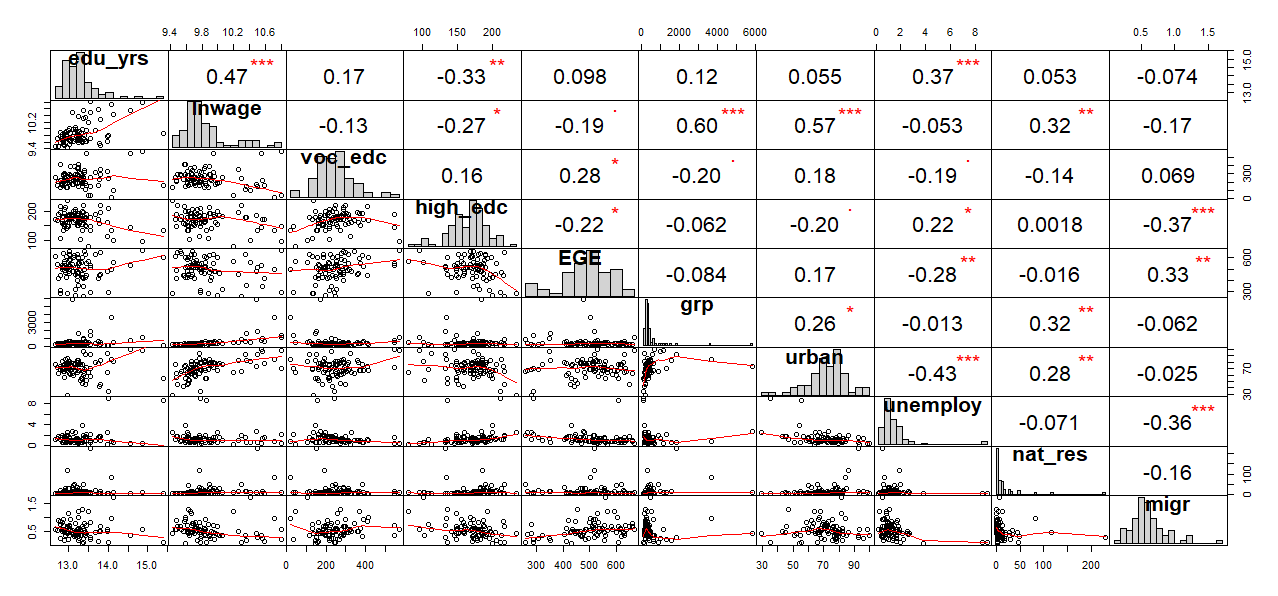
\includegraphics[width=8in]{cor_rgvars1.png}
			% plot 1
		\end{minipage}
		\caption{Correlations of Regional Level Variables with Wages and 
			Education}\label{fig:1.1}
	\end{figure}
\end{center}
\end{landscape}

\newpage
\begin{landscape}
	\begin{center}
		\begin{figure}[htbp!]
			\begin{minipage}[b]{1\linewidth}
				\centering
				\hspace*{-0.7in}
				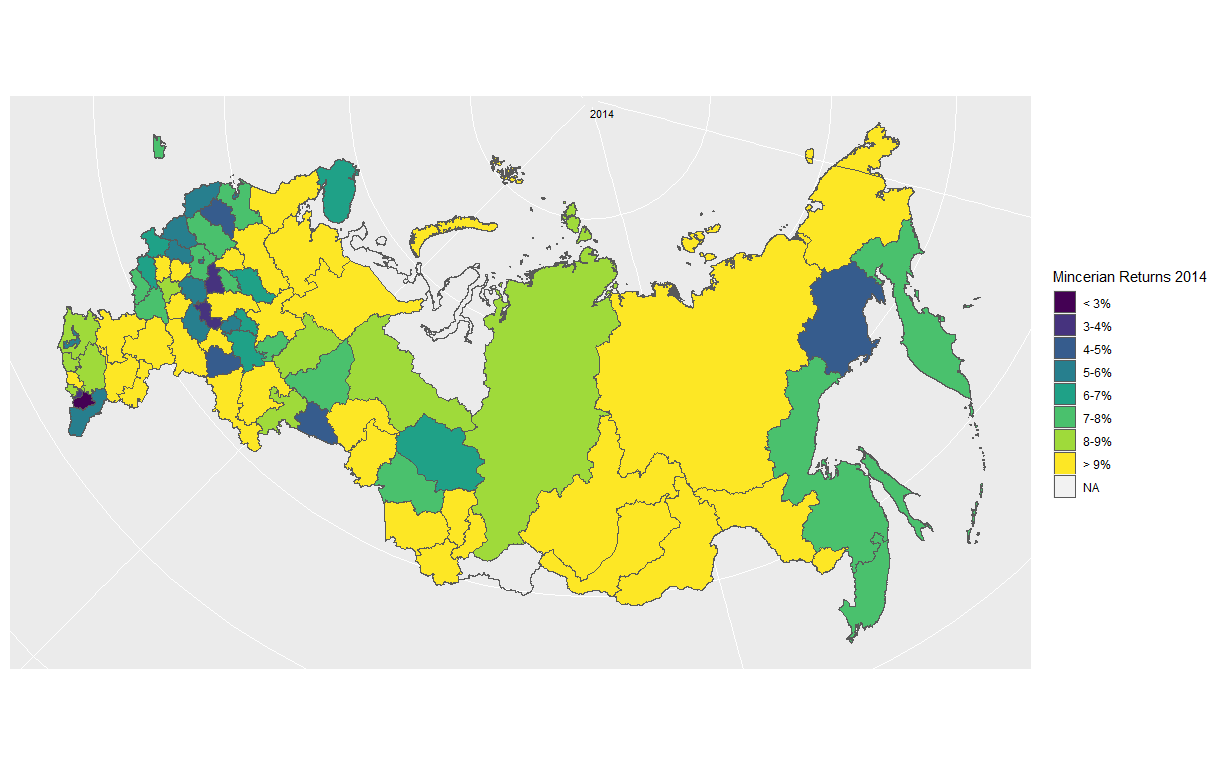
\includegraphics[width=7.5in]{map14.png}
				% plot 1
			\end{minipage}
			\caption{Mincerian Returns Basic Specification 
			2014}\label{fig:11.4}
		\end{figure}
	\end{center}
\end{landscape}

\begin{landscape}
	\begin{center}
		\begin{figure}[htbp!]
			\begin{minipage}[b]{1\linewidth}
				\centering
				\hspace*{-0.7in}
				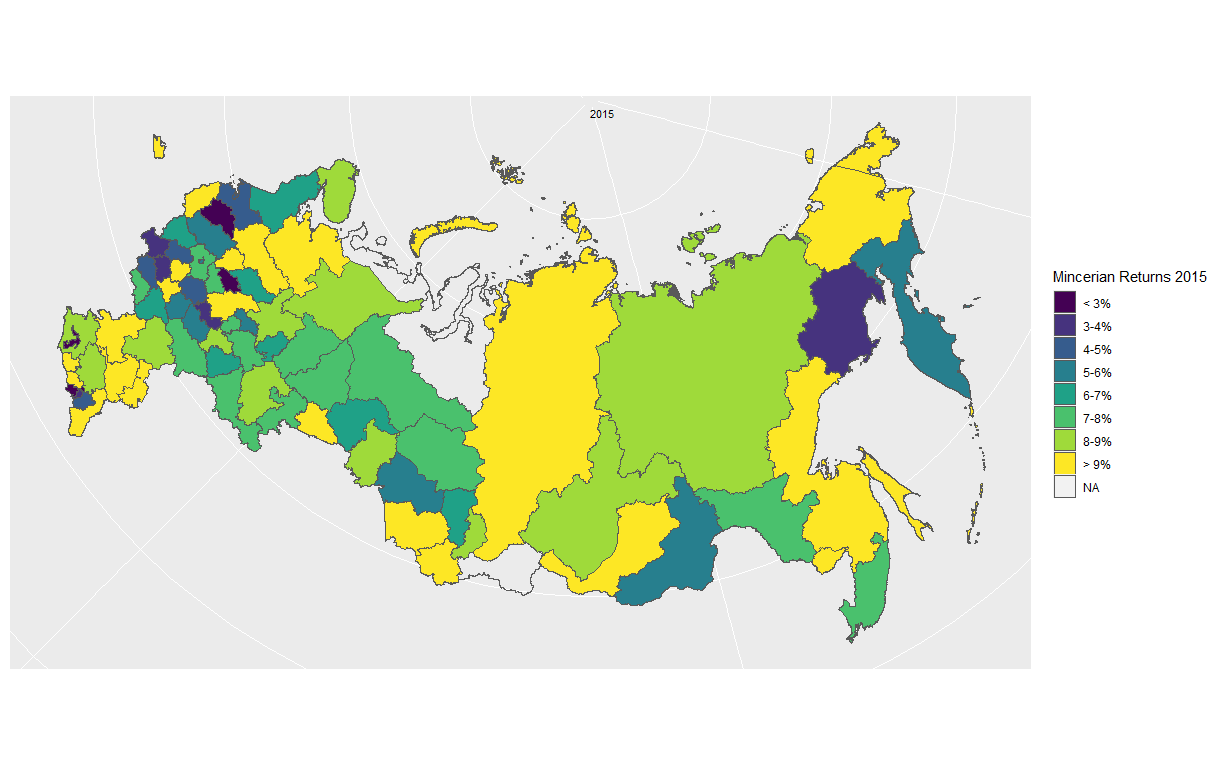
\includegraphics[width=7.5in]{map15.png}
				% plot 1
			\end{minipage}
			\caption{Mincerian Returns Basic Specification 
				2014}\label{fig:11.5}
		\end{figure}
	\end{center}
\end{landscape}

\begin{landscape}
	\begin{center}
		\begin{figure}[htbp!]
			\begin{minipage}[b]{1\linewidth}
				\centering
				\hspace*{-0.7in}
				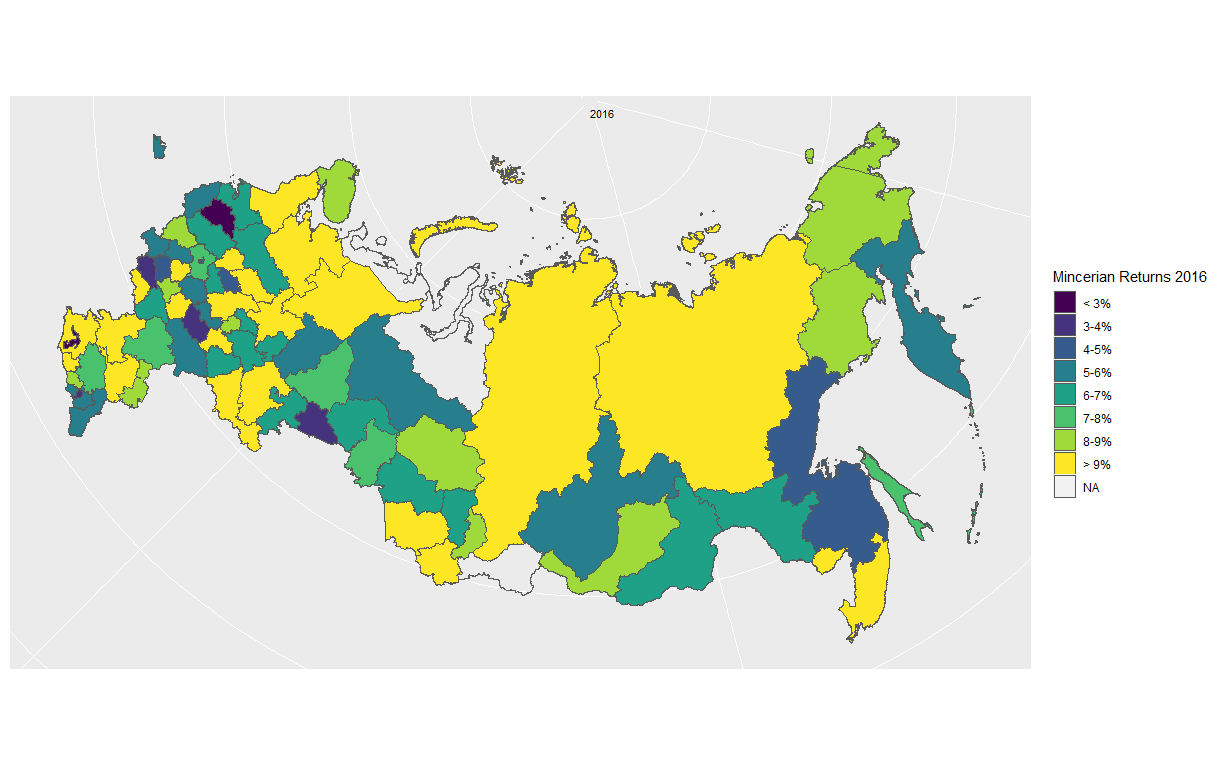
\includegraphics[width=7.5in]{map16.png}
				% plot 1
			\end{minipage}
			\caption{Mincerian Returns Basic Specification 
				2014}\label{fig:11.6}
		\end{figure}
	\end{center}
\end{landscape}

\begin{landscape}
	\begin{center}
		\begin{figure}[htbp!]
			\begin{minipage}[b]{1\linewidth}
				\centering
				\hspace*{-0.7in}
				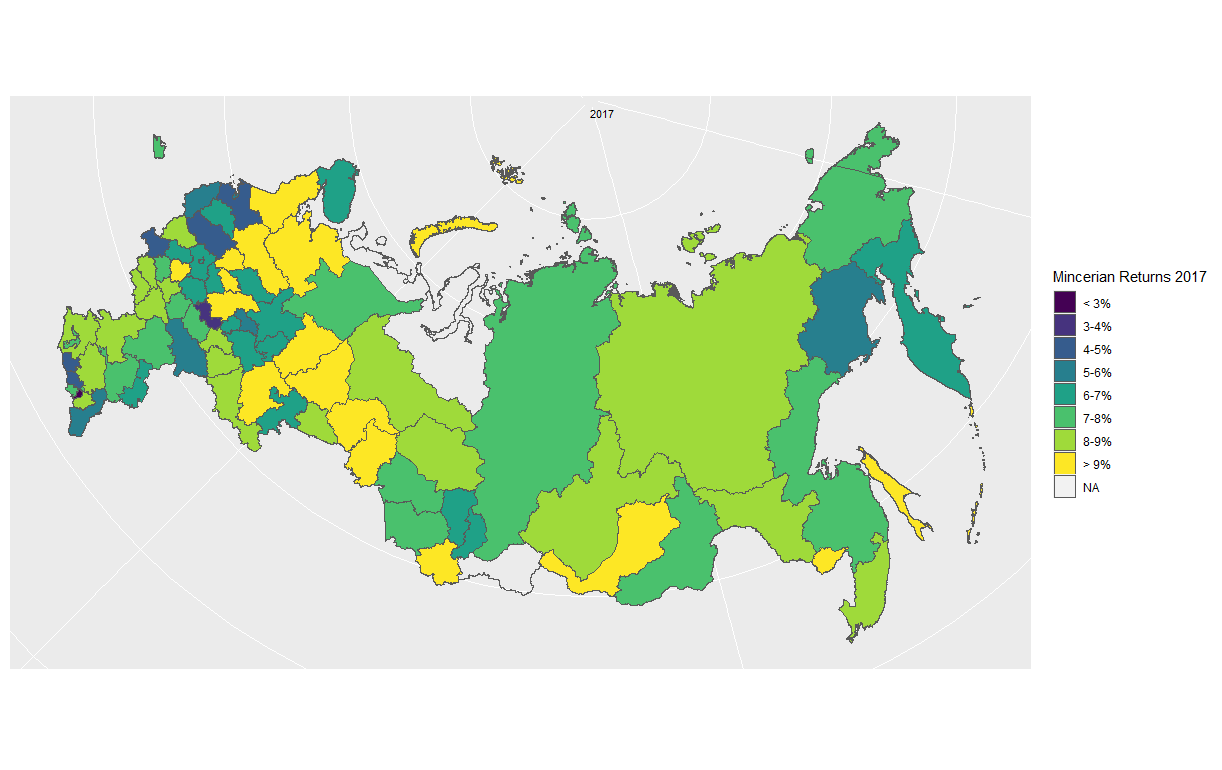
\includegraphics[width=7.25in]{map17.png}
				% plot 1
			\end{minipage}
			\caption{Mincerian Returns Basic Specification 
				2014}\label{fig:11.7}
		\end{figure}
	\end{center}
\end{landscape}

\begin{landscape}
	\begin{center}
		\begin{figure}[htbp!]
			\begin{minipage}[b]{1\linewidth}
				\centering
				\hspace*{-0.7in}
				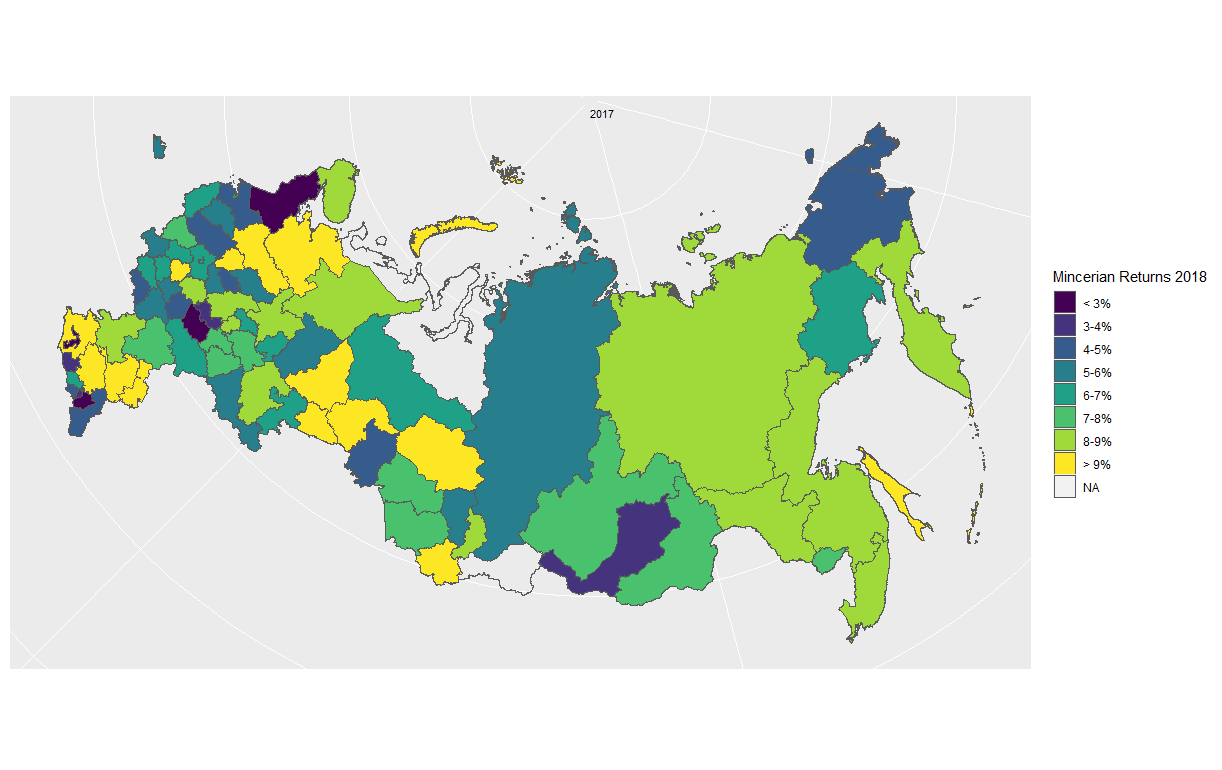
\includegraphics[width=7.25in]{map18.png}
				% plot 1
			\end{minipage}
			\caption{Mincerian Returns Basic Specification 
				2014}\label{fig:11.8}
		\end{figure}
	\end{center}
\end{landscape}



\end{document}
